\documentclass[a4paper, 10pt]{article}
\usepackage[margin=1in]{geometry}
\usepackage{amsfonts, amsmath, amssymb, amsthm}
\usepackage[none]{hyphenat}
\usepackage{fancyhdr} %create a custom header and footer
\usepackage[utf8]{inputenc}
\usepackage[english, main=ukrainian]{babel}
\usepackage{pgfplots}
\usepgfplotslibrary{fillbetween}
\usepackage{tikz}
\usepackage{graphicx}
\usepackage{caption}
\usepackage{float}
\usepackage{physics}
\usepackage[unicode]{hyperref}
\usepgfplotslibrary{polar}
\usepackage{ifthen}
\usetikzlibrary{spy, quotes, angles}
\usepackage{bbm}
\usetikzlibrary{babel}

\fancyhead{}
\fancyfoot{}
\parindent 0ex
\def\huge{\displaystyle}
\def\rightproof{$\boxed{\Rightarrow}$ }
\def\leftproof{$\boxed{\Leftarrow}$ }
\def\qed{$\blacksquare$}

\usepackage{pdfpages}

\newtheoremstyle{theoremdd}% name of the style to be used
  {\topsep}% measure of space to leave above the theorem. E.g.: 3pt
  {\topsep}% measure of space to leave below the theorem. E.g.: 3pt
  {\normalfont}% name of font to use in the body of the theorem
  {0pt}% measure of space to indent
  {\bfseries}% name of head font
  {}% punctuation between head and body
  { }% space after theorem head; " " = normal interword space
  {\thmname{#1}\thmnumber{ #2}\textnormal{\thmnote{ \textbf{#3}\\}}}

\theoremstyle{theoremdd}
\newtheorem{theorem}{Theorem}[subsection]

\theoremstyle{theoremdd}
\newtheorem{axiom}{Axiom}
  
\theoremstyle{theoremdd}
\newtheorem{definition}[theorem]{Definition}

\theoremstyle{theoremdd}
\newtheorem{samedef}[theorem]{Definition}

\theoremstyle{theoremdd}
\newtheorem{example}[theorem]{Example}

\theoremstyle{theoremdd}
\newtheorem{proposition}[theorem]{Proposition}

\theoremstyle{theoremdd}
\newtheorem{remark}[theorem]{Remark}

\theoremstyle{theoremdd}
\newtheorem{lemma}[theorem]{Lemma}

\theoremstyle{theoremdd}
\newtheorem{corollary}[theorem]{Corollary}

\makeatletter
\renewenvironment{proof}[1][Proof.\\]{\par
\pushQED{\hfill \qed}%
\normalfont \topsep6\p@\@plus6\p@\relax
\trivlist
\item\relax
{\bfseries
#1\@addpunct{.}}\hspace\labelsep\ignorespaces
}{%
\popQED\endtrivlist\@endpefalse
}
\makeatother

\newenvironment{pfMI}{\vspace*{-3mm} \textbf{\\ Proof MI. \\}}{\hfill $\blacksquare$}
\newenvironment{pfNoTh}{\textbf{Proof. \\}}{$\blacksquare$}

%delete

\begin{document}
\tableofcontents
\newpage

\section{Найпростіші геометричні фігури, їхні властивості}
\subsection{Точки та прямі}
Будуть три поняття, яким зазвичай не дають означення. Але малюнок дає представлення, що це.\\
Нижче представлені так звані \textbf{точки}. Їх ще називають найпростішою геометричною фігурою, що не можна розбити на частини.\\
Позначення: $A,B,C,\dots$
\begin{figure}[H]
\centering
\begin{tikzpicture}
\fill[black] circle (2pt) node[anchor = south] {$A$};
\fill[black] (1,1) circle (2pt) node[anchor = south] {$B$};
\end{tikzpicture}
\end{figure}

На наступному малюнку побудована \textbf{пряма}. Такий геометричний об'єкт матиме такі властивості.
\begin{axiom}
Через будь-які дві точки можна провести єдину пряму. Та яку б пряму ми не провели, існують точки, що належать цій прямій, та існують точки, що не належать цій прямій.
\end{axiom}
Позначення: $a,b,\dots$
\begin{figure}[H]
\centering
\begin{tikzpicture}
\draw[thick] (0,0)--(4,2) node at (0,0.5) {$a$};
\fill[black] (3,1.5) circle (2pt) node[anchor = south] {$A$};
\fill[black] (2,1) circle (2pt) node[anchor = south] {$B$};
\fill[black] (2,2) circle (2pt) node[anchor = south] {$C$};
\end{tikzpicture}
\caption*{В цьому малюнку маємо пряму $a$ або ще називають пряму $AB$, яка проведена через точки $A$,$B$.}
\end{figure}
Точку, яка належить прямій, позначатимемо так: $A \in a, B \in a$. \\
Точку, яка належить прямій, позначатимемо так: $C \notin a$.

\begin{definition}
Дві прямі (кажуть) \textbf{перетинаються}, якщо вони мають спільну точку.
\begin{figure}[H]
\centering
\begin{tikzpicture}
\draw[thick] (0,0)--(3,{3/2}) node at (0,0.5) {$a$};
\draw[thick] (0,2)--(2,0) node at (0.5,2) {$b$};

\fill[black] ({4/3},{2/3}) circle (2pt) node[anchor = south] {$O$};
\end{tikzpicture}
\caption*{Прямі $a,b$ мають спільну точку $O$. Отже, $a,b$ перетинаються.}
\end{figure}
\end{definition}

\begin{theorem}
Будь-які дві прямі, що перетинаються, мають лише одну спільну точку.
\end{theorem}

\begin{proof}
Задано дві прямі $a,b$, що перетинаються в спільній точці $O_1$.\\
!Припустимо, що $O_2$ -- ще одна спільна точка. Але тоді через ці дві точки $O_1,O_2$ проведені дві різні прямі (і саме $a,b$), коли за властивістю прямої, лише єдина пряма можлива. Суперечність!\\
(малюнку не буде, бо неможливо таку ситуацію уявити.)
\end{proof}

\subsection{Відрізок, довжина}
\begin{definition}
Задана пряма $a$, що проходить через т. $A,B$.\\
\textbf{Відрізком} назвемо частину прямої, що обмежена двома точками, які називають \textbf{кінцями}.\\
Позначення: $AB$
\begin{figure}[H]
\centering
\begin{tikzpicture}
\draw[thick] (0,0)--(4,0) node at (0,0.5) {$a$};
\draw[thick, red] (1,0)--(2,0);
\fill[black] (1,0) circle (2pt) node[anchor = south] {$A$};
\fill[black] (2,0) circle (2pt) node[anchor = south] {$B$};
\end{tikzpicture}
\caption*{Червоним маємо відрізок $AB$, де точки $A,B$ -- два кінця.}
\end{figure}
\end{definition}
Зрозуміло, що для кожних двох точок буде існувати єдиний відрізок, оскільки між ними існує єдина пряма.

\begin{definition}
Задан відрізок $AB$.\\
Точку $X$ назвемо \textbf{внутрішньою}, якщо вона лежить між кінцями відрізка.
\begin{figure}[H]
\centering
\begin{tikzpicture}
\draw[thick] (1,0)--(4,0);
\fill[black] (1,0) circle (2pt) node[anchor = south] {$A$};
\fill[black] (4,0) circle (2pt) node[anchor = south] {$B$};
\fill[black] (3,0) circle (2pt) node[anchor = south] {$X$};
\end{tikzpicture}
\caption*{Точка $X$ є внутрішьною відрізка $AB$.}
\end{figure}
Ще кажуть, що точка $X$ \textbf{розділяє} відрізок $AB$. Також кажуть, що точки $A,B$ \textbf{лежать по різні сторони} від точки $X$. Також кажуть, що точки $A,X$ \textbf{лежать по одну сторону} від точки $B$.
\end{definition}
Таким чином, відрізок $AB$ містить всі точки, що лежать між $A,B$, а також самі т. $A,B$.
\bigskip \\
До прямої дамо ще одну таку властивість. Вона про взаємне розташування точок на прямій.

\begin{axiom}
Серед трьох точок, що лежать на одній прямій, лише одна з них лежить між двома точками.
\end{axiom}

\iffalse
\begin{definition}
Задані відрізки $A_1B_1, A_2B_2$.\\
Їх назвемо \textbf{рівними}, якщо їх можна сумістити накладанням.\\
Позначення: $A_1B_1 = A_2B_2$.
\begin{figure}[H]
\centering
\begin{tikzpicture}
\draw[thick] (1,0)--(4,0);
\draw[thick] (1,-1)--(4,-1);
\fill[black] (1,0) circle (2pt) node[anchor = south] {$A_1$};
\fill[black] (4,0) circle (2pt) node[anchor = south] {$B_1$};
\fill[black] (1,-1) circle (2pt) node[anchor = south] {$A_2$};
\fill[black] (4,-1) circle (2pt) node[anchor = south] {$B_2$};
\end{tikzpicture}
\end{figure}

\begin{remark}
Можуть виникнути два можливих випадки під час накладання двох відрізків:\\
- $A_1$ співпадає з $A_2$ та $B_1$ співпадає з $B_2$;\\
- $A_1$ співпадає з $B_2$ та $B_1$ співпадає з $A_2$.
\end{remark}

У разі, якщо вони не рівні, то може виникнути один із двох випадків:\\
- відрізок $A_1B_1$ більший за $A_2B_2$: $A_1B_1 > A_2B_2$;\\
- відрізок $A_1B_1$ менший за $A_2B_2$: $A_1B_1 < A_2B_2$.
\end{definition}
\fi
Для того щоб виміряти \textbf{довжину} відрізка, треба буде задати \textbf{відрізки одиничної довжини}.\\
Зазвичай це: $1$см, $1$м, $1$дм.\\
Наприклад, вимірюють довжину відрізку, завдяки лінійці. Там відрізок одиничної довжини $1$см.\\
На відрізку має бути така властиість:\\
\iffalse
\begin{corollary}
Відрізки рівні тоді й тільки тоді, коли їхні довжини рівні.
\end{corollary}
\fi
\begin{axiom}
Кожен відрізок має довжину більше нуля. Якщо точка $C$ -- внутіршня точка відрізка $AB$, то довжину відрізка $AB$ можна знати таким чином:
\begin{align*}
AB = AC + CB
\end{align*}
\begin{figure}[H]
\centering
\begin{tikzpicture}
\draw[thick] (1,0)--(4,0);
\fill[black] (1,0) circle (2pt) node[anchor = south] {$A$};
\fill[black] (4,0) circle (2pt) node[anchor = south] {$B$};
\fill[black] (3,0) circle (2pt) node[anchor = south] {$C$};
\end{tikzpicture}
\end{figure}
\end{axiom}

\begin{example}
Нехай відомо, що точки $A,B,C$ лежать на одній прямій. Також відомо, що $AB = 4.3$см, $AC=7.5$см, $BC = 3.2$см.\\
Уже відомо, що точно серед цих точок лише одна лежить між іншими.\\
Якщо $A$ лежить між $B,C$, то тоді $BC = BA + AC$, але тоді $3.2 = 4.3 + 7.5$, що хибно.\\
Якщо $C$ лежить між $A,B$, то тоді $AB = AC + CB$, але тоді $4.3 = 7.5 + 3.2$, що хибно.\\
Єдиний варіант тоді залишається -- це коли точка $B$ лежить між $A,C$.
\end{example}

\begin{definition}
\textbf{Відстанню} між точками $A,B$ називають довжину відрізка $AB$.\\
Якщо ці точки збігаються, то відстань $= 0$.
\end{definition}

\begin{definition}
\textbf{Серединою} відрізка $AB$ називають таку внутрішню точку $C$, що
\begin{align*}
AC = CB
\end{align*}
\begin{figure}[H]
\centering
\begin{tikzpicture}
\draw[thick] (1,0)--(4,0);
\fill[black] (1,0) circle (2pt) node[anchor = south] {$A$};
\fill[black] (2.5,0) circle (2pt) node[anchor = south] {$C$};
\fill[black] (4,0) circle (2pt) node[anchor = south] {$B$};
\draw (1.75,-2pt)--(1.75,2pt);
\draw (3.25,-2pt)--(3.25,2pt);
\end{tikzpicture}
\caption*{Двома міні палками позначають, що ці відрізки рівні за довжиною.}
\end{figure}
\end{definition}

\subsection{Півплощина}
\textbf{Площину} можна сприймати як стіл нескінченної довжини, де малюються всі геометричні фігури. Якщо намалювати пряму (яка нескінченна), то планується, щоб вона мала таку властивість:
\begin{axiom}
Пряма розбиває площину на дві півплощини.
\begin{figure}[H]
\centering
\begin{tikzpicture}
\draw[thick] (-2,-1)--(2,1);
\fill[black] (-1,1) circle (2pt) node[anchor = south] {$A$};
\fill[black] (-0.5,0.5) circle (2pt) node[anchor = south] {$B$};
\fill[black] (0.5,1) circle (2pt) node[anchor = south] {$C$};
\fill[black] (0.5,-1) circle (2pt) node[anchor = north] {$D$};
\draw (-1,1)--(-0.5,0.5);
\draw (0.5,1)--(0.5,-1);
\end{tikzpicture}
\caption*{На малюнку точки $A,B,C$ лежать на одній півплощині. Водночас точки $C,D$ лежать на різних півплощинах. Відрізок $AB$ не перетинає пряму, тому що $A,B$ лежать на одній півплощині. Відрізок $CD$ водночас перетинає пряму, оскільки $C,D$ лежать на різних півплощинах.}
\end{figure}
\end{axiom}

\subsection{Промінь, кут, вимірювання кутів}
\begin{definition}
Задано пряму $AB$. Позначимо деяку точку $O$.\\
\textbf{Променем} або \textbf{півпрямою} називають частину прямої, всі точки яких лежать по одну сторону з точкою $O$. Точка $O$ називається \textbf{початком} променя.
\begin{figure}[H]
\centering
\begin{tikzpicture}
\draw[thick] (1,0)--(4,0);
\fill[black] (1,0) circle (0pt) node[anchor = south] {$A$};
\fill[black] (4,0) circle (0pt) node[anchor = south] {$B$};
\fill[black] (2,0) circle (2pt) node[anchor = south] {$O$};
\end{tikzpicture}
\qquad
\begin{tikzpicture}
\draw[thick] (1,0)--(5,0);
\fill[black] (2,0) circle (2pt) node[anchor = south] {$A$};
\fill[black] (4,0) circle (2pt) node[anchor = south] {$B$};
\fill[black] (1,0) circle (2pt) node[anchor = south] {$O$};
\end{tikzpicture}
\caption*{На першому малюнку два промені: $OA$ та $OB$. На другому один промінь: $OA$ або $OB$ (можна один з двох варіантів назвати).}
\end{figure}
\end{definition}

\begin{definition}
Два промені називаються \textbf{доповняльними}, якщо вони мають спільний початок і лежать на одній прямій.
\end{definition}
У попередньому малюнку, першому, промені $AO$, $OB$ - доповняльні. Тому що спільний початок $O$ та, об'єднавши, отримаємо пряму $AB$.

\begin{example}
Задано відрізок $AB$ та точка $C$, що лежить на відрізку. Серед півпроменів $AB,AC,CA,CB$ назвати ці, що збігаються, та ці, що доповняльні.\\
Точка $C$ лежить між $A,B$. Отже, точка $A$ уже не може лежати між $B,C$. Отже, $B,C$ лежать по одну сторону від точки $A$. Тому промені $AB,AC$ збігаються.\\
Оскільки точка $C$ лежить між $A,B$, то тоді $A,B$ лежать по різні сторони від $C$. Також якщо об'єднати $CA,CB$, то ми отримаємо пряму $AB$. Отже, $CA,CB$ -- доповняльні.
\end{example}

\begin{definition}
Задано два промені зі спільним початком $O$.\\
\textbf{Кутом} будемо називати фігуру, що утворена двома променями.\\
Позначення: $\angle BOA$, $\angle AOB$ або $\angle O$.
\begin{figure}[H]
\centering
\begin{tikzpicture}
\coordinate (a) at (2,-1);
\coordinate (b) at (0,0);
\coordinate (c) at (3,2);
[draw, angle eccentricity=1.5] {angle=a--b--c};
\draw[thick] (b)--(c);
\draw[thick] (b)--(a);
\fill[black] (b) circle (2pt) node [anchor = south] {$O$};
\fill[black] (c) circle (0pt) node[anchor = south] {$A$};
\fill[black] (a) circle (0pt) node[anchor = south] {$B$};
\end{tikzpicture}
\caption*{Промені $OA,OB$ назвемо \textbf{сторонами кута}, а точку $O$ назвемо \textbf{вершиною кута}.}
\end{figure}
\end{definition}
Кут можна розглядати або всередині двох променів, або зовні. Зазвичай розглядається перший варіант.

\begin{definition}
Кут назвемо \textbf{розгорнутим}, якщо сторони кутів -- доповняльні промені.
\begin{figure}[H]
\centering
\begin{tikzpicture}
\coordinate (a) at (1,0);
\coordinate (b) at (2,0);
\coordinate (c) at (4,0);
\pic [draw] {angle=c--b--a};
\draw[thick] (a)--(c);
\fill[black] (a) circle (0pt) node[anchor = south] {$A$};
\fill[black] (c) circle (0pt) node[anchor = south] {$B$};
\fill[black] (b) circle (2pt) node[anchor = north] {$O$};
\end{tikzpicture}
\end{figure}
\end{definition}

\iffalse
\begin{definition}
Задані два кута $\angle A_1O_1B_1, \angle A_2O_2B_2$\\
Їх назвемо \textbf{рівними}, якщо їх можна сумістити накладанням.\\
Позначення: $\angle A_1O_1B_1 = \angle A_2O_2B_2$
\begin{figure}[H]
\centering
\begin{tikzpicture}
\draw[thick] (0,0)--(2,0);
\draw[thick] (0,0)--(2,1);

\draw[thick] (4,0)--(6,0);
\draw[thick] (4,0)--(6,1);
\fill[black] (0,0) circle (0pt) node [anchor = south] {$O_1$};
\fill[black] (2,0) circle (0pt) node[anchor = south] {$A_1$};
\fill[black] (2,1) circle (0pt) node[anchor = south] {$B_1$};
\fill[black] (4,0) circle (0pt) node [anchor = south] {$O_2$};
\fill[black] (6,0) circle (0pt) node[anchor = south] {$A_2$};
\fill[black] (6,1) circle (0pt) node[anchor = south] {$B_2$};
\end{tikzpicture}
\end{figure}
У разі, якщо вони не рівні, то може виникнути один із двох випадків:\\
- кут $\angle A_1O_1B_1$ більший за $\angle A_2O_2B_2$: $\angle A_1O_1B_1 > \angle A_2O_2B_2$;\\
- кут $\angle A_1O_1B_1$ менший за $\angle A_2O_2B_2$: $\angle A_1O_1B_1 < \angle A_2O_2B_2$.
\end{definition}

\textbf{Axiom.} Для кута $ABC$ та променя $B_1C_1$ існує єдиний кут $A_1B_1C_1$, який дорівнює куту $ABC$. Причому т. $C_1$ лежить у заданій півплощині відносно прямої $B_1C_1$.
\fi
Для того щоб виміряти \textbf{міру} кута, це можна зробити за допомогою транспортира, що повертає значення в градусах. Є ще так звані мінути (не хвилини), що дорівнюють $\dfrac{1}{60}$ градуса.
\begin{axiom}
Кожен кут має градусну міру більше нуля. Розгорнутий кут дорівнює $180^\circ$. Якщо в $\angle AOB$ є промінь $OC$, що проходить між сторонами $OA,OB$, то градусну міру $\angle AOB$ можна записати таким чином:
\begin{align*}
\angle AOB = \angle AOC + \angle COB
\end{align*}
\begin{figure}[H]
\centering
\begin{tikzpicture}
\coordinate (a) at (2,-1);
\coordinate (b) at (0,0);
\coordinate (c) at (3,2);
\coordinate (d) at (2,0);
\draw[thick] (b)--(c);
\draw[thick] (b)--(a);
\draw[thick] (b)--(d);
\fill[black] (b) circle (0pt) node [anchor = south] {$O$};
\fill[black] (c) circle (0pt) node[anchor = south] {$A$};
\fill[black] (a) circle (0pt) node[anchor = south] {$B$};
\fill[black] (d) circle (0pt) node[anchor = south] {$C$};
\end{tikzpicture}
\end{figure}
\end{axiom}

\subsection{Відкладення відрізків та кутів}
\begin{axiom}
На кожну півпряму від початкової точки можна відкласти лише один відрізок заданої довжини.
\begin{figure}[H]
\centering
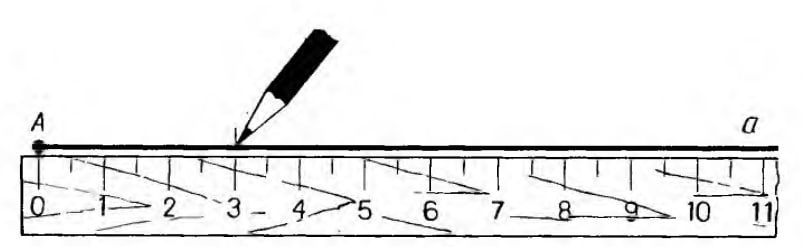
\includegraphics[scale=0.5]{ruler(from_Pogorelov).jpg}
\caption*{Маємо якусь пряму $a$ та точку відліку $A$. Від неї ми можемо відкласти єдиний відрізок довжини $3$см. Це зазвичай робиться за допомогою лінійки.}
\end{figure}
\end{axiom}

\begin{axiom}
Від кожній півпрямій в задану півплощину можна відкласти лише один кут із заданою градусною мірою, менший за $180^\circ$.
\begin{figure}[H]
\centering
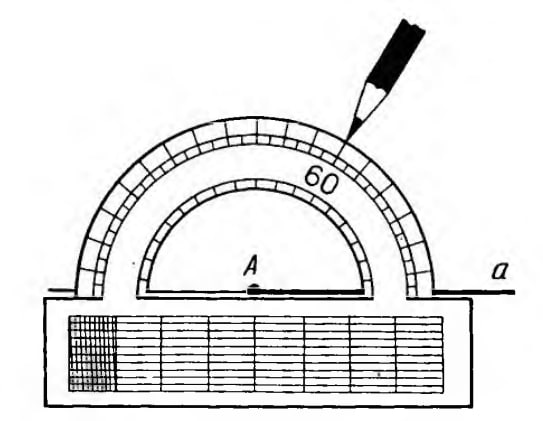
\includegraphics[scale=0.5]{protractor(from_Pogorelov).jpg}
\caption*{Маємо якусь півпряму $a$, що починається з точки $A$. Півпряма розбиває площину на дві частини. На одну з півплощи можна відкласти єдиний кут градусної міри $60^\circ$. Це зазвичай робиться за допомогою транспортира.}
\end{figure}
\end{axiom}

\subsection{Основні види кутів}
\begin{definition}
\textbf{Бісектрисою} кута називають промінь з початком у вершині кута, що ділить цей кут на два рівних кути.
\begin{figure}[H]
\centering
\begin{tikzpicture}
\coordinate (a) at (2,-1);
\coordinate (b) at (0,0);
\coordinate (c) at (3,2);
\coordinate (d) at (2,0.2);
\pic [draw, angle eccentricity=1.5] {angle=a--b--c};
\draw[thick] (b)--(c);
\draw[thick] (b)--(a);
\draw[thick] (b)--(d);
\fill[black] (b) circle (2pt) node [anchor = south] {$O$};
\fill[black] (c) circle (0pt) node[anchor = south] {$A$};
\fill[black] (a) circle (0pt) node[anchor = south] {$B$};
\fill[black] (d) circle (0pt) node[anchor = south] {$D$};
\end{tikzpicture}
\caption*{$OD$ - бісектриса кута $AOB$. Звідси маємо $\angle AOD = \angle BOD$.}
\end{figure}
\end{definition}

\iffalse
Для того щоб виміряти \textbf{величину} кута, треба буде задати \textbf{одиничний кут}.\\
Зазвичай це $1^{\circ}$ - це можна отримати, якщо розгорнутий кут розділити на $180$ рівних кутів.\\
Є ще $1' = \dfrac{1}{60}^{\circ}$ - одна мінута (не хвилина).

\begin{corollary}
Розгорнутий кут дорівнює $180^{\circ}$.
\end{corollary}

\begin{corollary}
Кути рівні тоді й тільки тоді, коли їхні кутові величини рівні.
\end{corollary}
\fi

\begin{definition} Задано кут $\angle AOB$.
Кут називається:\\
- \textbf{прямим}, якщо $\angle AOB = 90^{\circ}$;\\
- \textbf{гострим}, якщо $\angle AOB < 90^{\circ}$;\\
- \textbf{тупим}, якщо $\angle AOB > 90^{\circ}$.
\begin{figure}[H]
\centering
\begin{tikzpicture}
\draw[thick] (0,0)--(2,0);
\draw[thick] (0,0)--(0,2);
\fill[black] (0,0) circle (0pt) node [anchor = east] {$O$};
\fill[black] (2,0) circle (0pt) node[anchor = south] {$A$};
\fill[black] (0,2) circle (0pt) node[anchor = south] {$B$};
\end{tikzpicture}
\qquad
\begin{tikzpicture}
\draw[thick] (0,0)--(2,0);
\draw[thick] (0,0)--(2,1);
\fill[black] (0,0) circle (0pt) node [anchor = south] {$O$};
\fill[black] (2,0) circle (0pt) node[anchor = south] {$A$};
\fill[black] (2,1) circle (0pt) node[anchor = south] {$B$};
\end{tikzpicture}
\qquad
\begin{tikzpicture}
\draw[thick] (0,0)--(2,0);
\draw[thick] (0,0)--(-2,1);
\fill[black] (0,0) circle (0pt) node [anchor = south] {$O$};
\fill[black] (2,0) circle (0pt) node[anchor = south] {$A$};
\fill[black] (-2,1) circle (0pt) node[anchor = south] {$B$};
\end{tikzpicture}
\end{figure}
\end{definition}

\iffalse
\textbf{Axiom.} Якщо промінь $OC$ ділить кут $\angle AOB$ на два інших кути $\angle AOC$, $\angle COD$, то кут $\angle AOB$ можна знайти таким чином:
\begin{align*}
\angle AOB = \angle AOC + \angle COB
\end{align*} 
\begin{figure}[H]
\centering
\begin{tikzpicture}
\coordinate (a) at (2,-1);
\coordinate (b) at (0,0);
\coordinate (c) at (3,2);
\coordinate (d) at (2,0);
\draw[thick] (b)--(c);
\draw[thick] (b)--(a);
\draw[thick] (b)--(d);
\fill[black] (b) circle (0pt) node [anchor = south] {$O$};
\fill[black] (c) circle (0pt) node[anchor = south] {$A$};
\fill[black] (a) circle (0pt) node[anchor = south] {$B$};
\fill[black] (d) circle (0pt) node[anchor = south] {$C$};
\end{tikzpicture}
\end{figure}
\fi

\subsection{Суміжні та вертикальні кути}
\begin{definition}
Два кути називають \textbf{суміжними}, якщо одна сторона спільна, а також два інших промені є доповняльними.
\begin{figure}[H]
\centering
\begin{tikzpicture}
\draw[thick] (0,0)--(3,0);
\draw[thick] (1,0)--(2,1);
\fill[black] (1,0) circle (0pt) node [anchor = south] {$O$};
\fill[black] (0,0) circle (0pt) node[anchor = south] {$A$};
\fill[black] (2,1) circle (0pt) node[anchor = south] {$B$};
\fill[black] (3,0) circle (0pt) node[anchor = south] {$C$};
\end{tikzpicture}
\caption*{Тут кути $\angle AOB, \angle COB$ -- суміжні, оскільки $OB$ спільна сторона та $AO,OC$ -- доповняльні.}
\end{figure}
\end{definition}

\begin{theorem}
Сума суміжних кутів $= 180^{\circ}$.
\end{theorem}

\begin{proof}
Повернімось до малюнку. Хочемо: $\angle AOB + \angle COB = 180^{\circ}$.\\
Ці кути -- суміжні. Отже, $OA,OB$ -- доповняльні. А тому $\angle AOC = 180^{\circ}$, бо він -- розгорнутий.\\
А також $\angle AOC = \angle AOB + \angle COB$. Остаточно, $\angle AOB + \angle COB = 180^{\circ}$.
\end{proof}

\begin{definition}
Два кути називають \textbf{вертикальними}, якщо сторони одного кута -- доповняльні промени других сторін.
\begin{figure}[H]
\centering
\begin{tikzpicture}
\draw[thick] (0,0)--(3,0);
\draw[thick] (0,-1)--(2,1);
\fill[black] (1,0) circle (0pt) node [anchor = south] {$O$};
\fill[black] (0,0) circle (0pt) node[anchor = south] {$A$};
\fill[black] (2,1) circle (0pt) node[anchor = south] {$B$};
\fill[black] (3,0) circle (0pt) node[anchor = south] {$C$};
\fill[black] (0,-1) circle (0pt) node[anchor = south] {$D$};
\end{tikzpicture}
\caption*{Тут кути $\angle AOD, \angle COB$ - вертикальні, бо сторони $AO,OD$ -- доповняльні до $OC, OB$.}
\end{figure}
\end{definition}

\begin{theorem}
Вертикальні кути рівні.
\end{theorem}

\begin{proof}
Повернімось до малюнку. Хочемо: $\angle AOD = \angle COB$.\\
$\angle AOD, \angle AOB$ -- суміжні, а тому $\angle AOD + \angle AOB = 180^{\circ} \implies \angle AOB = 180^{\circ} - \angle AOD$.\\
$\angle AOB, \angle BOC$ -- суміжні, а тому $\angle AOB + \angle COB = 180^{\circ} \\ \implies \angle COB = 180^{\circ} - \angle AOB = 180^{\circ} - (180^{\circ} - \angle AOD) = \angle AOD$.
\end{proof}

\subsection{Перпендикулярні прямі}
\begin{definition}
Задані прямі $a,b$.\\
Дві прямі називають \textbf{перпендикулярними}, якщо при їхньому перетині утвориться прямий кут.\\
Позначення: $a \perp b$.
\begin{figure}[H]
\centering
\begin{tikzpicture}
\draw[thick] (-1,0)--(2,0) node[anchor = south] {$a$};
\draw[thick] (0,-1)--(0,2) node[anchor = east] {$b$};
\draw (0,0) rectangle (0.25,0.25);
\end{tikzpicture}
\end{figure}
Якщо один кут прямий, то тоді суміжний та вертикальний кути -- також прямі.
\end{definition}

\begin{definition}
\textbf{Кутом між прямими} $AD,BC$ будемо називати величину гострого кута, що утворився в результаті перетину.
\begin{figure}[H]
\centering
\begin{tikzpicture}
\draw[thick] (0,0)--(3,0);
\draw[thick] (0,-1)--(2,1);
\fill[black] (1,0) circle (0pt) node [anchor = south] {$O$};
\fill[black] (0,0) circle (0pt) node[anchor = south] {$A$};
\fill[black] (2,1) circle (0pt) node[anchor = south] {$B$};
\fill[black] (3,0) circle (0pt) node[anchor = south] {$D$};
\fill[black] (0,-1) circle (0pt) node[anchor = south] {$C$};
\end{tikzpicture}
\caption*{Тобто $\angle AOC$ або $\angle BOD$ -- кут між прямими $AD,BC$}.
\end{figure}
\end{definition}

\begin{definition} Задані відрізки $AB,CD$.\\
Вони називаються \textbf{перпендикулярними}, якщо вони лежать на перпендикулярних прямих.
\begin{figure}[H]
\centering
\begin{tikzpicture}
\draw[thick] (-1,0)--(3,0);
\draw[thick, red] (1,0)--(2,0);
\draw[thick] (0,-1)--(0,2.5);
\draw[thick, red] (0,0.5)--(0,2);
\draw (0,0) rectangle (0.25,0.25);
\fill[black] (1,0) circle (2pt) node [anchor = south] {$A$};
\fill[black] (2,0) circle (2pt) node [anchor = south] {$B$};
\fill[black] (0,0.5) circle (2pt) node [anchor = east] {$C$};
\fill[black] (0,2) circle (2pt) node [anchor = east] {$D$};
\end{tikzpicture}
\end{figure}
\end{definition}
Можна також розглядати перпендикулярність двох променів, променя та відрізка, прямої та променя, відрізка та прямої.

\begin{definition}
Задана пряма $a$ та перпендикуляр $AB$, причому $B \in a$.\\
Тоді точка $B$ називається \textbf{основою перпендикуляра}. Довжина $AB$ називається \textbf{відстанню} від т. $A$ до прямої $a$.
\begin{figure}[H]
\centering
\begin{tikzpicture}
\draw[thick] (-1,0)--(3,0) node[anchor = south] {$a$};
\draw[thick, red] (0,0)--(0,2);
\draw (0,0) rectangle (0.25,0.25);
\fill[black] (0,0) circle (2pt) node [anchor = north] {$B$};
\fill[black] (0,2) circle (2pt) node [anchor = east] {$A$};
\end{tikzpicture}
\end{figure}
\end{definition}
Можна довжину $AB$ ще називати відстанню від т. $A$ до променя $BR$, якщо $BR \in a$; або відстанюю від т. $A$ до відрізка $SG$, якщо $SG \in a$.

\begin{theorem}
Через кожну точку прямої можна провести єдину пряму, що перпендикулярна до даної.
\end{theorem}

\begin{proof}
Нехай є пряма $AB$, на якій я позначу точку $M$. Відкладемо від промення $MB$ кут $CMB$, який буде прямим. Отже, $CM \perp AB$.\\
!Припустимо, що існує ще одна пряма, якась пряма $DM$, що перпендикулярна $AB$. Нехай точка $D$ лежить у тій самій півплощині відносно прямої $AB$, що й точка $C$. Отримали прямий кут, який відкладений також від прямої $AB$. Але від неї в заданій півплощині можна відкласти лише єдиний кут -- суперечність!
\end{proof}
\newpage


\section{Трикутники}
\subsection{Основні означення. Висота, медіана, бісектриса}
\begin{definition}
Задано три точки $A,B,C$, що не лежать на одній прямій З'єднаємо ці точки відрізками $AB,BC,CA$.\\
Утворена геометрична фігура називається \textbf{трикутником}.\\
Позначення: $\Delta ABC$.
\begin{figure}[H]
\centering
\begin{tikzpicture}
\draw[thick] (0,0)--(3,2)--(5,0)--(0,0);
\fill[black] (0,0) circle (0pt) node [anchor = north] {$A$};
\fill[black] (3,2) circle (0pt) node [anchor = south] {$B$};
\fill[black] (5,0) circle (0pt) node [anchor = north] {$C$};
\end{tikzpicture}
\end{figure}
Точки трикутника називаються \textbf{вершинами}, а відрізки трикутника називаються \textbf{сторонами}.
\end{definition}

Кут $BAC$ (наприклад) ще називають \textbf{кутом трикутника при вершині $A$}.

\begin{definition} Задано трикутник $\Delta ABC$.\\
\textbf{Периметром трикутника} назвемо таку величину:
\begin{align*}
P_{\Delta ABC} = AB + BC + CA
\end{align*}
Тобто периметром трикутника називають суму всіх сторін трикутника.
\end{definition}

\iffalse
\begin{definition}
Задано два трикутника $\Delta A_1B_1C_1$, $\Delta A_2B_2C_2$.\\
Ці трикутники називаються \textbf{рівними}, якщо їх можна сумістити накладанням.\\
Позначення: $\Delta A_1B_1C_1 = \Delta A_2B_2C_2$.
\end{definition}
\fi

\begin{definition}
Два трикутника $\Delta ABC$ та $\Delta DEF$  називаються \textbf{рівними}, якщо відповідні сторони та відповідні кути рівні. При цьому відповідні кути мають лежати проти відповідних сторін. Тобто:
\begin{align*}
\angle A = \angle D \qquad \angle B = \angle E \qquad \angle C = \angle F \\
AB = DE \qquad BC = EF \qquad CA = FD 
\end{align*}
Позначення: $\Delta ABC = \Delta DEF$.
\begin{figure}[H]
\centering
\begin{tikzpicture}
\pgfmathsetmacro{\point}{2*0.0352777778}
\draw[thick] (0,0)--(3,2)--(5,0)--(0,0);
\fill[black] (0,0) circle (0pt) node [anchor = north] {$A$};
\fill[black] (3,2) circle (0pt) node [anchor = south] {$B$};
\fill[black] (5,0) circle (0pt) node [anchor = north] {$C$};

\draw[thick] (2.5,-2pt)--(2.5,2pt);
%\draw[thick] ({4-\point},{4-\point-3})--({4+\point},{4+\point-3});
%\draw[thick] ({3.8-\point},{3.8-\point-3})--({3.8+\point},{3.8+\point-3});
\draw (1.5,-1pt)--(1.5,1pt);
\end{tikzpicture}
\qquad
\begin{tikzpicture}
\draw[thick] (0,0)--(2,3)--(0,5)--(0,0);
\fill[black] (0,0) circle (0pt) node [anchor = north] {$D$};
\fill[black] (2,3) circle (0pt) node [anchor = west] {$E$};
\fill[black] (0,5) circle (0pt) node [anchor = south] {$F$};
\end{tikzpicture}
\end{figure}
(TODO: доробити малюнок).
\end{definition}

\subsubsection{Існування трикутника, що рівний заданому}
Нехай маємо $\Delta ABC$ та промінь $a$. Перемістимо $\Delta ABC$ таким чином, щоб вершина $A$ сумістилася з початком променя, вершина $B$ потрапила на промінь $a$, вершина $C$ потрапила в задану півплощину відносно променя $a$ та його продовження.\\
Вершини нового трикутника позначимо $A_1,B_1,C_1$.\\
$\Delta A_1B_1C_1 = \Delta ABC$.
\begin{axiom}
Який б не був трикутник, існує рівний йому трикутник в заданому розташуванні відносно заданій півпрямій.
\begin{figure}[H]
\centering
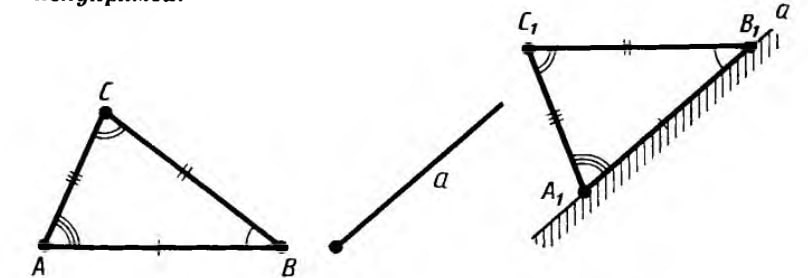
\includegraphics[scale=0.5]{construct_triangle(from_Pogorelov).jpg}
\end{figure}
\end{axiom}

\iffalse
\begin{corollary}
$\Delta A_1B_1C_1 = \Delta A_2B_2C_2 \iff$ кожний кут та кожна сторона першого трикутника дорівнює кожному куту та кожній стороні другого трикутника.
\end{corollary}

\textbf{Axiom.} Для заданого трикутника $ABC$ та заданого променя $A_1M$ існує трикутник $A_1B_1C_1$, який дорівнює $ABC$. Причому сторона $A_1B_1$ належить променю $A_1M$.
\bigskip \\
\textit{Треба трошки відволіктись та повернутись до перпендикулярних прямих.}
\fi

\begin{theorem}
Через точку, що не належить прямій, можна провести іншу єдину пряму, що перпендикулярна першій прямій.
\end{theorem}

\begin{proof}
Розглянемо пряму $MN$ та точку $O \not\in MN$. Покажемо, що ми можемо провести пряму через т. $O$, що перпендикулярна $MN$.\\
Для початку ми створимо кут $\angle OMN$. А далі відкладемо від променя $MN$ єдиний кут $O_1MN$ так, щоб $\angle OMN = \angle O_1MN$. Причому точку $O_1$ ми оберемо так, щоб $OM=O_1M$.\\
Проведемо пряму $OO_1$, яка перетинається з прямою $MN$. Позначу точкою перетину точку $A$. Лишилось довести, що $\angle MAO = 90^\circ$.\\
Маємо $\Delta OMA$ та промінь $MA$. Тоді за \textbf{Axiom}, можна знайти рівний трикутний $\Delta O_2MA = \Delta O_1MA$. Із рівності отримаємо, що $\angle AMO_1 = \angle AMO_2$, а тому точка $O_2$ належить куту $\angle AMO_1$. Також із рівності отримаємо, що $MO_1 = MO_2$, тоді $MO_2 = MO$. Таким чином, точка $O_1$ співпадає з точкою $O_2$, а тому звідси $\Delta O_1MA, \Delta O_2MA$ збігаються. Оскільки $\Delta O_1AM = \Delta OAM$, то тоді $\angle MAO_1 = \angle MAO$, причому ці кути суміжні. Отже, $\alpha MAO = 90^\circ$. Все, довели.
\bigskip \\
!Припустимо, що через т. $O \not \in MN$ можна провести другу пряму, що перпендикулярна $MN$. (TODO).
\end{proof}

\begin{definition}
\textbf{Висотою} трикутника називають перпендикуляр, що опущений із вершини трикутника на пряму, яка містить протилежну сторону
\begin{figure}[H]
\centering
\begin{tikzpicture}
\draw[thick] (0,0)--(3,2)--(5,0)--(0,0);
\fill[black] (0,0) circle (0pt) node [anchor = north] {$A$};
\fill[black] (3,2) circle (0pt) node [anchor = south] {$B$};
\fill[black] (5,0) circle (0pt) node [anchor = north] {$C$};
\draw[thick] (3,2)--(3,0);
\fill[black] (3,0) circle (0pt) node [anchor = north] {$H$};
\draw (3,0) rectangle (3.25,0.25);
\end{tikzpicture}
\qquad
\begin{tikzpicture}
\draw[thick] (0,0)--(3,2)--(2,0)--(0,0);
\draw[dashed] (2,0)--(3.5,0);
\fill[black] (0,0) circle (0pt) node [anchor = north] {$A$};
\fill[black] (3,2) circle (0pt) node [anchor = south] {$B$};
\fill[black] (2,0) circle (0pt) node [anchor = north] {$C$};
\draw[thick] (3,2)--(3,0);
\fill[black] (3,0) circle (0pt) node [anchor = north] {$H$};
\draw (3,0) rectangle (3.25,0.25);
\end{tikzpicture}
\end{figure}
\end{definition}

\begin{definition}
\textbf{Медіаною} трикутника називають відрізок, що сполучає вершину трикутника з серединою протилежної сторони.
\begin{figure}[H]
\centering
\begin{tikzpicture}
\draw[thick] (0,0)--(3,2)--(5,0)--(0,0);
\fill[black] (0,0) circle (0pt) node [anchor = north] {$A$};
\fill[black] (3,2) circle (0pt) node [anchor = south] {$B$};
\fill[black] (5,0) circle (0pt) node [anchor = north] {$C$};
\draw[thick] (3,2)--(2.5,0);
\fill[black] (2.5,0) circle (0pt) node [anchor = north] {$M$};
\end{tikzpicture}
\end{figure}
\end{definition}

\begin{definition}
\textbf{Бісектрисою} трикутника називають бісектрису трикутника, що сполучає вершину трикутника з точкою протилежної сторони.
\begin{figure}[H]
\centering
\begin{tikzpicture}
\coordinate (a) at (2,-1);
\coordinate (b) at (0,0);
\coordinate (c) at (3,2);
\coordinate (d) at (2.4,0.2);
\pic [draw, angle eccentricity=1.5] {angle=a--b--c};
\draw[thick] (b)--(c);
\draw[thick] (b)--(a);
\draw[thick] (b)--(d);
\draw[thick] (c)--(a);
\fill[black] (b) circle (0pt) node [anchor = south] {$A$};
\fill[black] (c) circle (0pt) node[anchor = south] {$B$};
\fill[black] (a) circle (0pt) node[anchor = south west] {$C$};
\fill[black] (d) circle (0pt) node[anchor = south west] {$L$};
\end{tikzpicture}
\end{figure}
\end{definition}

\subsection{Ознаки рівності трикутників}
\begin{theorem}[Перша ознака]
Нехай дві сторони та кут між ними одного трикутника дорівнює відповідно двом сторонам та куту між ними другого трикутника. Тоді ці трикутники рівні.
\end{theorem}

\begin{proof}
Задані $\Delta A_1B_1C_1$, $\Delta A_2B_2C_2$. Нехай буде $A_1B_1 = A_2B_2$, $B_1C_1 = B_2C_2$, $\angle B_1 = \angle B_2$.
\begin{figure}[H]
\centering
\begin{tikzpicture}
\coordinate (a) at (0,0);
\coordinate (b) at (1,2);
\coordinate (c) at (3,0);
\pic [draw, angle eccentricity=1.5] {angle=a--b--c};
\draw[thick] (a)--(b)--(c)--(a);
\fill[black] (a) circle (0pt) node [anchor = north] {$A_1$};
\fill[black] (b) circle (0pt) node [anchor = south] {$B_1$};
\fill[black] (c) circle (0pt) node [anchor = north] {$C_1$};
\draw (0.4,1.05)--(0.6,0.95);
\draw (1.9,0.95)--(2.1,1.05);
\draw (2,0.85)--(2.2,0.95);
\end{tikzpicture}
\qquad
\begin{tikzpicture}
\coordinate (a) at (0,0);
\coordinate (b) at (1,2);
\coordinate (c) at (3,0);
\pic [draw, angle eccentricity=1.5] {angle=a--b--c};
\draw[thick] (a)--(b)--(c)--(a);
\fill[black] (a) circle (0pt) node [anchor = north] {$A_2$};
\fill[black] (b) circle (0pt) node [anchor = south] {$B_2$};
\fill[black] (c) circle (0pt) node [anchor = north] {$C_2$};
\draw (0.4,1.05)--(0.6,0.95);
\draw (1.9,0.95)--(2.1,1.05);
\draw (2,0.85)--(2.2,0.95);
\end{tikzpicture}
\end{figure}
Оскільки $\angle B_1 = \angle B_2$, то ми накладемо промені $\Delta A_1B_1C_1$ на $\Delta A_2B_2C_2$ таким чином, щоб $B_1A_1$ сумістився з $B_2A_2$ та $B_1C_1$ сумістився з $B_2C_2$.\\
Оскільки $A_1B_1 = A_2B_2$, $B_1C_1 = B_2C_2$, то тоді сторони теж сумістяться. Отже, трикутники повністю сумістяться $\Rightarrow \Delta A_1B_1C_1 = \Delta A_2B_2C_2$.
\end{proof}

\begin{definition}
\textbf{Серединним перпендикуляром} відрізка називають пряму, що перпендикулярна до відрізка та проходить через його середину.
\begin{figure}[H]
\centering
\begin{tikzpicture}
\draw[thick, red] (-1,0)--(3,0) node[anchor = south] {$a$};
\draw[thick] (1,-1)--(1,1);
\draw (1,0) rectangle (1.25,0.25);
\fill[black] (1,1) circle (2pt) node [anchor = east] {$B$};
\fill[black] (1,-1) circle (2pt) node [anchor = east] {$A$};
\draw (1cm-2pt,0.5)--(1cm+2pt,0.5);
\draw (1cm-2pt,-0.5)--(1cm+2pt,-0.5);
\end{tikzpicture}
\end{figure}
\end{definition}

\begin{theorem}
Кожна точка серединного перпендикуляра відрізка рівновіддалена від кінців його відрізка.
\end{theorem}

\begin{proof}
Задано пряму $a$ - серединний перпендикуляр відрізка $AB$. Оберемо будь-яку точку $X \in a$. Хочемо довести, що $AX = BX$.
\begin{figure}[H]
\centering
\begin{tikzpicture}
\draw[thick] (-1,-0.5)--(1,-0.5);
\draw[thick,red] (0,-1)--(0,1.5) node[anchor = south east] {$a$};
\draw (0,-0.5) rectangle (0.25,-0.25);
\fill[black] (-1,-0.5) circle (2pt) node [anchor = north] {$A$};
\fill[black] (1,-0.5) circle (2pt) node [anchor = north] {$B$};
\draw (0.5,-0.5-0.1)--(0.5,-0.5+0.1); \draw (-0.5,-0.5-0.1)--(-0.5,-0.5+0.1);
\fill[black] (0,1) circle (2pt) node [anchor = west] {$X$};
\draw (0,1)--(-1,-0.5); \draw (0,1)--(1,-0.5);
\node at (0.2,-0.7) {$M$};
\end{tikzpicture}
\end{figure}
Із точки $X$ проведемо $AX$ та $BX$. На малюнку будуть $\Delta AMX$ та $\Delta BMX$. Про них відомо, що $AM = MB$, існує спільна сторона $MX$ та $\angle AMX = \angle BMX$. Отже, за першою ознакою, $\Delta AMX = \Delta BMX$.\\
Остаточно, $AX = BX$.
\end{proof}

\begin{theorem}[Друга ознака]
Нехай сторона та прилеглі до неї кути одного трикутника дорівнюють стороні та прилеглим до неї кутам другого трикутника. Тоді ці трикутники рівні.
\end{theorem}

\begin{proof}
Задані $\Delta A_1B_1C_1$, $\Delta A_2B_2C_2$. Нехай буде $A_1B_1 = A_2B_2$, \hspace{0.5cm} $\angle A_1 = \angle A_2$, $\angle B_1 = \angle B_2$.
\begin{figure}[H]
\centering
\begin{tikzpicture}
\coordinate (a) at (0,0);
\coordinate (b) at (1,2);
\coordinate (c) at (3,0);
\pic [draw, angle eccentricity=1.5] {angle=a--b--c};
\pic [draw, angle eccentricity=1.5] {angle=c--a--b};
\draw[thick] (a)--(b)--(c)--(a);
\fill[black] (a) circle (0pt) node [anchor = north] {$A_1$};
\fill[black] (b) circle (0pt) node [anchor = south] {$B_1$};
\fill[black] (c) circle (0pt) node [anchor = north] {$C_1$};
\draw (0.4,1.05)--(0.6,0.95);
\end{tikzpicture}
\qquad
\begin{tikzpicture}
\coordinate (a) at (0,0);
\coordinate (b) at (1,2);
\coordinate (c) at (3,0);
\pic [draw, angle eccentricity=1.5] {angle=a--b--c};
\pic [draw, angle eccentricity=1.5] {angle=c--a--b};
\draw[thick] (a)--(b)--(c)--(a);
\fill[black] (a) circle (0pt) node [anchor = north] {$A_2$};
\fill[black] (b) circle (0pt) node [anchor = south] {$B_2$};
\fill[black] (c) circle (0pt) node [anchor = north] {$C_2$};
\draw (0.4,1.05)--(0.6,0.95);
\end{tikzpicture}
\end{figure}
Оскільки $A_1B_1 = A_2B_2$, то накладемо $\Delta A_1B_1C_1$ на $\Delta A_2B_2C_2$ таким чином, щоб $C_1,C_2$ лежали на одній півплощині відносно $A_2B_2$. Оскільки $\angle A_1 = \angle A_2$, $\angle B_1 = \angle B_2$, то звідси промені $B_1C_1,B_2C_2$ співпадають та промені $A_1C_1,A_2C_2$ співпадають. Отже, точка $C_1$ суміститься з $C_2$.\\
Таким чином, трикутники повністю сумістяться, а тому $\Delta A_1B_1C_1 = \Delta A_2B_2C_2$.
\end{proof}

\textit{Ще сюди повернемось}

\subsection{Рівнобедрені трикутники}
\begin{definition}
\textbf{Рівнобедреним трикутником} називають трикутник з двома однаковими сторонами.
\begin{figure}[H]
\centering
\begin{tikzpicture}
\coordinate (a) at (0,0);
\coordinate (b) at (1,2);
\coordinate (c) at (2,0);
\draw[thick] (a)--(b)--(c)--(a);
\fill[black] (a) circle (0pt) node [anchor = north] {$A$};
\fill[black] (b) circle (0pt) node [anchor = south] {$B$};
\fill[black] (c) circle (0pt) node [anchor = north] {$C$};
\draw (0.4,1.05)--(0.6,0.95);
\draw (1.4,0.95)--(1.6,1.05);
\end{tikzpicture}
\end{figure}
Сторони $AB,BC$ називають \textbf{бічними сторонами}. Сторону $AC$ називають \textbf{основою}.\\
Точку $B$ називають \textbf{вершиною рівнобедреного трикутника} .
\end{definition}

\begin{definition}
\textbf{Рівностороннім трикутником} назвемо трикутник з всіма рівними сторонами.
\end{definition}

\begin{theorem}[Властивості]
1. Кути при основі рівні;\\
2. Бісектриса, що проведена до основи, є медіаною та висотою.\\
\textit{Вказівка: із точки вершини провести бісектрису.}
\end{theorem}

\begin{corollary}[Наслідок з властивостей]
1. Проти рівних сторін лежать рівні кути;\\
2. Бісектриса, висота, медіана, що проведені з вершини, збігаються;\\
3. У рівностороннього трикутника всі кути рівні $60^\circ$;\\
4. У рівностороннього трикутника бісектриса, висота, медіана, що проведени з однієї з трьох вершин, збігаються.
\end{corollary}

\begin{definition}
\textbf{Різностороннім трикутником} назвемо трикутник, де всі довжини сторін різні.
\end{definition}

\begin{theorem}[Ознака рівнобедреного трикутника 1]
Якщо медіана трикутника є висотою, то даний трикутник - рівнобедрений.
\end{theorem}

\begin{proof}
Задано $\Delta ABC$ та $BH$ - медіана та висота одночасно.
\begin{figure}[H]
\centering
\begin{tikzpicture}
\coordinate (a) at (0,0);
\coordinate (b) at (1,2);
\coordinate (c) at (2,0);
\draw[thick] (a)--(b)--(c)--(a);
\fill[black] (a) circle (0pt) node [anchor = north] {$A$};
\fill[black] (b) circle (0pt) node [anchor = south] {$B$};
\fill[black] (c) circle (0pt) node [anchor = north] {$C$};
\draw (b)--(1,0) node[anchor = north] {$H$};
\draw (1,0) rectangle (1.25,0.25);
\draw (0.5,-2pt)--(0.5,2pt);
\draw (1.5,-2pt)--(1.5,2pt);
\end{tikzpicture}
\end{figure}
Із умови задачі ми маємо, що $BH$ - серединний перпендикуляр відрізка $AC$. Тоді за \textbf{Th. 2.2.3.}, $AB = AC$. Отже, $\Delta ABC$ - рівнобедрений.
\end{proof}

\begin{theorem}[Ознака рівнобедреного трикутника 2]
Якщо бісектриса трикутниика є висотою, то даний трикутник - рівнобедрений.
\end{theorem}

\begin{proof}
Задано $\Delta ABC$ та $BH$ - бісектриса та висота одночасно.
\begin{figure}[H]
\centering
\begin{tikzpicture}
\coordinate (a) at (0,0);
\coordinate (b) at (1,2);
\coordinate (c) at (2,0);
\coordinate (d) at (1,0);
\draw[thick] (a)--(b)--(c)--(a);
\fill[black] (a) circle (0pt) node [anchor = north] {$A$};
\fill[black] (b) circle (0pt) node [anchor = south] {$B$};
\fill[black] (c) circle (0pt) node [anchor = north] {$C$};
\draw (b)--(d) node[anchor = north] {$H$};
\draw (1,0) rectangle (1.25,0.25);
\pic [draw, angle eccentricity=1.5] {angle=a--b--d};
\pic [draw, angle eccentricity=1.5, angle radius = 0.7cm] {angle=d--b--c};
\end{tikzpicture}
\end{figure}
Із умови задачі ми маємо, що $\angle ABH = \angle CBH$, $\angle AHB = \angle CHB$ та спільна сторона $BH$. Отже, за II ознаком рівності, $\Delta AHB = \Delta CHB$, а тому $AB = BC$. Отже, $\Delta ABC$ - рівнобедрений.
\end{proof}

\begin{theorem}[Ознака рівнобедреного трикутника 3]
Якщо в трикутнику два кути рівні, то даний трикутник - рівнобедрений.
\end{theorem}

\begin{proof}
Задано $\Delta ABC$ та $\angle A = \angle C$.\\
Проведемо серединний перпендикуляр $a$ відрізка $AC$. Хочеться довести, що $a$ проходить через т. $B$, щоб скористатись \textbf{Th. 2.3.6.}\\
!Припустимо, що $a$ НЕ проходить через т. $B$. Позначимо точку перетину сторони $AB$ як $M$, а центр відрізка $AC$ як $H$.\\
Через точку $C$ проведемо пряму $CM$. Тоді за \textbf{Th. 2.2.3}, $AM = MC$. Отже, $\Delta AMC$ - рівнобедрений. Тоді за наслідком, $\angle MAC = \angle MCA$. Нам також відомо, що $\angle C = \angle A = \angle MAC$, тому основна властивість кутів не виконується. Суперечність!\\
До речі, $a$ може перетинати $BC$, а не $AB$, але аналогічно можна отримати суперечність.\\
Отже, $a$ проходить через $B$, а тому $a$ - висота й медіана $\Delta ABC$ одночасно. Отже, $\Delta ABC$ - рівнобедрений.
\end{proof}

\begin{corollary}
У трикутнику проти рівних кутів лежать рівні сторони.
\end{corollary}

\begin{corollary}
Якщо в трикутнику всі кути рівні, то даний трикутник - рівносторонній.
\end{corollary}

\begin{theorem}[Ознака рівності трикутника 4]
Якщо медіана трикутника є бісектрисою, то даний трикутник - рівнобедрений.
\end{theorem}

\begin{proof}
Задано $\Delta ABC$ та $BH$ - медіана та бісектриса одночасно.
\begin{figure}[H]
\centering
\begin{tikzpicture}
\coordinate (a) at (0,0);
\coordinate (b) at (1,2);
\coordinate (c) at (2,0);
\coordinate (d) at (1,0);
\draw[thick] (a)--(b)--(c)--(a);
\fill[black] (a) circle (0pt) node [anchor = north] {$A$};
\fill[black] (b) circle (0pt) node [anchor = south] {$B$};
\fill[black] (c) circle (0pt) node [anchor = north] {$C$};
\draw (b)--(d) node[anchor = north] {$H$};
\draw (0.5,-2pt)--(0.5,2pt);
\draw (1.5,-2pt)--(1.5,2pt);
\pic [draw, angle eccentricity=1.5] {angle=a--b--d};
\pic [draw, angle eccentricity=1.5, angle radius = 0.7cm] {angle=d--b--c};
\end{tikzpicture}
\end{figure}
$BH$ уявимо як промінь. На ній позначимо точку $M$ таким чином, щоб $BH = HM$. А далі проведемо пряму $MA$. Буде щось ось таке:
\begin{figure}[H]
\centering
\begin{tikzpicture}
\coordinate (a) at (0,0);
\coordinate (b) at (1,2);
\coordinate (c) at (2,0);
\coordinate (d) at (1,0);
\coordinate (e) at (1,-2);
\draw[thick] (a)--(b)--(c)--(a);
\fill[black] (a) circle (0pt) node [anchor = north] {$A$};
\fill[black] (b) circle (0pt) node [anchor = south] {$B$};
\fill[black] (c) circle (0pt) node [anchor = north] {$C$};
\draw (b)--(d) node[anchor = north west] {$H$};
\draw (0.5,-2pt)--(0.5,2pt);
\draw (1.5,-2pt)--(1.5,2pt);
\pic [draw, angle eccentricity=1.5] {angle=a--b--d};
\pic [draw, angle eccentricity=1.5, angle radius = 0.7cm] {angle=d--b--c};

\draw[dashed] (d)--(e)--(a);
\fill[black] (e) circle (0pt) node [anchor = north] {$M$};

\draw (1-0.1,0.9)--(1+0.1,0.9);
\draw (1-0.1,1.1)--(1+0.1,1.1);

\draw (1-0.1,-0.9)--(1+0.1,-0.9);
\draw (1-0.1,-1.1)--(1+0.1,-1.1);
\end{tikzpicture}
\end{figure}
Маємо $BH = BM$ та $AH = HC$. А ще $\angle AHM = \angle CHB$ як вертикальні кути. Отже, за I ознакою рівності, $\Delta AHM = \Delta CHB$.\\
Тоді $AM = BC$, а також $\angle AMH = \angle HBC \overset{BM \text{- бісектриса}}{=} \angle ABH$. Якщо подивитись на $\Delta MAB$, то маємо, що $\angle AMB = \angle ABM$. Звідси $\Delta MAB$ - рівнобедрений за ознакою, а тому $AM = AB$.\\
$AM = BC, AM = AB \implies AB = BC$. Отже, $\Delta ABC$ - рівнобедрений.
\end{proof}

\textit{Повернімось до ознак рівності трикутника}

\begin{theorem}[Третя ознака]
Нехай три сторони одного трикутника дорівнюють трьом сторонам другого трикутника. Тоді ці трикутники рівні.
\end{theorem}

\begin{proof}
Задано $\Delta A_1B_1C_1, \Delta A_2B_2C_2$. Нехай $A_1B_1 = A_2B_2$, $B_1C_1 = B_2C_2$, $C_1A_1 = C_2A_2$.
\begin{figure}[H]
\centering
\begin{tikzpicture}
\coordinate (a) at (0,0);
\coordinate (b) at (1,2);
\coordinate (c) at (3,0);
\draw[thick] (a)--(b)--(c)--(a);
\fill[black] (a) circle (0pt) node [anchor = north] {$A_1$};
\fill[black] (b) circle (0pt) node [anchor = south] {$B_1$};
\fill[black] (c) circle (0pt) node [anchor = north] {$C_1$};
\draw (0.4,1.05)--(0.6,0.95);
\draw (1.9,0.95)--(2.1,1.05);
\draw (2,0.85)--(2.2,0.95);
\draw[red] (1.5,-2pt)--(1.5,2pt);
\end{tikzpicture}
\qquad
\begin{tikzpicture}
\coordinate (a) at (0,0);
\coordinate (b) at (1,2);
\coordinate (c) at (3,0);
\draw[thick] (a)--(b)--(c)--(a);
\fill[black] (a) circle (0pt) node [anchor = north] {$A_2$};
\fill[black] (b) circle (0pt) node [anchor = south] {$B_2$};
\fill[black] (c) circle (0pt) node [anchor = north] {$C_2$};
\draw (0.4,1.05)--(0.6,0.95);
\draw (1.9,0.95)--(2.1,1.05);
\draw (2,0.85)--(2.2,0.95);
\draw[red] (1.5,-2pt)--(1.5,2pt);
\end{tikzpicture}
\end{figure}
Оскільки $A_1C_1 = A_2C_2$, то ми можемо їх накласти. Зробимо це таким чином:
\begin{figure}[H]
\centering
\begin{tikzpicture}
\coordinate (a) at (0,0);
\coordinate (b) at (1,2);
\coordinate (c) at (3,0);
\coordinate (d) at (1,-2);
\draw[thick] (a)--(b)--(c)--(a);
\draw[thick] (a)--(d)--(c);
\fill[black] (a) circle (0pt) node [anchor = north east] {$A_1 (A_2)$};
\fill[black] (b) circle (0pt) node [anchor = south] {$B_1$};
\fill[black] (c) circle (0pt) node [anchor = north west] {$C_1 (C_2)$};
\fill[black] (d) circle (0pt) node [anchor = north] {$B_2$};
\draw (0.4,1.05)--(0.6,0.95);
\draw (0.4,-1.05)--(0.6,-0.95);

\draw (1.9,0.95)--(2.1,1.05);
\draw (2,0.85)--(2.2,0.95);
\draw (1.9,-0.95)--(2.1,-1.05);
\draw (2,-0.85)--(2.2,-0.95);
\draw[red] (1.5,-2pt)--(1.5,2pt);

\draw[dashed] (b)--(d);
\end{tikzpicture}
\end{figure}
А далі проведемо $B_1B_2$. Матимемо два рівнобедрений трикутника: $\Delta B_2A_1B_1$ та $\Delta B_2C_1B_1$. У них кути при основі рівні, тобто $\angle A_1B_2B_1 = \angle A_1B_1B_2$ та $\angle B_2B_1C_1 = \angle B_1B_2C_1$.\\
Тому $\angle B_1 = \angle A_1B_1B_2 + \angle B_2B_1C_1 = \angle A_1B_2B_1 + \angle B_1B_2C_1 = \angle B_2$.\\
Отже, за I ознакою рівності, $\Delta A_2B_2C_2 = \Delta A_1B_1C_1$.
\bigskip \\
Це ми розглянули випадок з гострокутними трикутниками. Якщо трикутники будуть прямокутними та тупокутними, то під час накладання двох трикутників картина вже буде іншою:
\begin{figure}[H]
\centering
\begin{tikzpicture}
\coordinate (a) at (0,0);
\coordinate (b) at (-1,2);
\coordinate (c) at (3,0);
\coordinate (d) at (-1,-2);
\draw[thick] (a)--(b)--(c)--(a);
\draw[thick] (a)--(d)--(c);
\fill[black] (a) circle (0pt) node [anchor = north east] {$A_1 (A_2)$};
\fill[black] (b) circle (0pt) node [anchor = south] {$B_1$};
\fill[black] (c) circle (0pt) node [anchor = north west] {$C_1 (C_2)$};
\fill[black] (d) circle (0pt) node [anchor = north] {$B_2$};
\end{tikzpicture}
\qquad
\begin{tikzpicture}
\coordinate (a) at (0,0);
\coordinate (b) at (0,2);
\coordinate (c) at (3,0);
\coordinate (d) at (0,-2);
\draw[thick] (a)--(b)--(c)--(a);
\draw[thick] (a)--(d)--(c);
\fill[black] (a) circle (0pt) node [anchor = north east] {$A_1 (A_2)$};
\fill[black] (b) circle (0pt) node [anchor = south] {$B_1$};
\fill[black] (c) circle (0pt) node [anchor = north west] {$C_1 (C_2)$};
\fill[black] (d) circle (0pt) node [anchor = north] {$B_2$};
\end{tikzpicture}
\end{figure}
Але доведення аналогічні першому випадку.
\end{proof}

\begin{theorem}
Якщо точка рівновіддалена від кінців відрізка, то ця точка належить серединном перпендикуляру відрізка.
\end{theorem}

\begin{proof}
Задано точку $X$ та відрізок $AB$. Відомо, що $XA =XB$.\\
На відрізку $AB$ оберемо середину $M$. А далі проведемо $XM$. Тоді $\Delta AXM = \Delta BXM$ за ІІІ ознакою. Тоді $\angle XMA = \angle XMB$, а ще вони - суміжні, тому $\angle XMA = 90^\circ$.\\
Таким чином, $XM \perp AB$, тому $X$ належить серединному перпендикуляру.
\begin{figure}[H]
\centering
\begin{tikzpicture}
\coordinate (a) at (0,0);
\coordinate (b) at (1,2);
\coordinate (c) at (2,0);
\draw[thick] (a)--(b)--(c)--(a);
\fill[black] (a) circle (0pt) node [anchor = north] {$A$};
\fill[black] (b) circle (0pt) node [anchor = south] {$X$};
\fill[black] (c) circle (0pt) node [anchor = north] {$B$};
\draw (0.4,1.05)--(0.6,0.95);
\draw (1.4,0.95)--(1.6,1.05);
\draw[dashed] (b)--(1,0) node [anchor = north] {$M$};

\draw[red] (0.5,-2pt)--(0.5,2pt);
\draw[red] (1.5,-2pt)--(1.5,2pt);
\end{tikzpicture}
\end{figure}
\end{proof}
\newpage

\section{Паралельні прямі та знову про трикутники}
\subsection{Паралельні прямі}
\begin{definition}
Задано прямі $a,b$.\\
Ці прямі називаються \textbf{паралельними}, якщо вони не перетинаються.\\
Позначення: $a \parallel b$.
\begin{figure}[H]
\centering
\begin{tikzpicture}
\draw[thick] (0,0)--(2,0) node[anchor = south] {$a$};
\draw[thick] (0,1)--(2,1) node[anchor = south] {$b$};
\end{tikzpicture}
\end{figure}
\end{definition}

Для паралельних прямих існує властивість:
\begin{axiom}
Через точку, що не належить прямій, можна провести єдину пряму, паралельна заданій прямій.
\end{axiom}

\begin{definition}
Задані відрізки $AB,CD$.\\
Вони називаються \textbf{паралельними}, якщо вони лежать на паралельних прямих.
\begin{figure}[H]
\centering
\begin{tikzpicture}
\draw[thick] (0,0)--(2,0) node[anchor = south west] {$a$};
\draw[thick] (0,1)--(2,1) node[anchor = south west] {$b$};

\fill[black] (0.5,0) circle (2pt) node [anchor = south] {$A$};
\fill[black] (1.5,0) circle (2pt) node [anchor = south] {$B$};
\fill[black] (0.2,1) circle (2pt) node [anchor = south] {$C$};
\fill[black] (1.8,1) circle (2pt) node [anchor = south] {$D$};

\draw[red,thick] (0.5,0)--(1.5,0);
\draw[red,thick] (0.2,1)--(1.8,1);
\end{tikzpicture}
\end{figure}
\end{definition}

\begin{theorem}[Ознака паралельності]
Дві прямі, що перпендикулярні третій прямій, паралельні.
\end{theorem}

\begin{proof}
Задані відрізки $a,b,c$. Відомо, що $a \perp c, b \perp c$.\\
\begin{figure}[H]
\centering
\begin{tikzpicture}
\draw[thick] (0,0)--(2,0) node[anchor = south] {$a$};
\draw[thick] (0,1)--(2,1) node[anchor = south] {$b$};
\draw[thick] (0.5,1.5)--(0.5,-0.5) node[anchor = north] {$c$};
\draw (0.5,1) rectangle (0.75,1.25);
\draw (0.5,0) rectangle (0.75,0.25);
\end{tikzpicture}
\end{figure}
!Припустимо, що $a \not\parallel b$, тобто вони перетинаються в т. $M$. Тоді через т. $M$, що не належить прямій $c$, проходять дві прямі, що перпендикулярні: це $a$ та $b$. Але відомо, що така пряма - єдина. Суперечність!\\
Таким чином, $a \parallel b$.
\end{proof}

\begin{corollary}
Через точку, що не належить прямій, можна провести іншу єдину пряму, що паралельна першій прямій.
\end{corollary}

\begin{proof}
Маємо пряму $a$ та т. $M \not\in a$. Відомо, що через т. $M$ ми можемо провести пряму $b \perp a$. А також через цю ж т. $M$ прямій $b$ ми можемо провести пряму $c \perp b$.\\
Таким чином, ми отримали, що $a \parallel c$, а точка $M \in c$.\\
Єдиність прямої буде відповідати аксіома нижче.
\end{proof}

\begin{theorem}
Якщо перші дві прямі паралельні третій, то перші дві прямі паралельні між собою.
\end{theorem}

\begin{proof}
Задано $a \parallel c$, $b \parallel c$.\\
\begin{figure}[H]
\centering
\begin{tikzpicture}
\draw[thick] (0,0)--(2,0) node[anchor = south] {$a$};
\draw[thick] (0,1)--(2,1) node[anchor = south] {$b$};
\draw[thick] (0,-1)--(2,-1) node[anchor = south] {$c$};
\end{tikzpicture}
\end{figure}
!Припустимо, що $a \not\parallel b$, тоді вони перетинаються в т. $M$. Тоді через т. $M$, що не належить прямій $c$, проходять дві прямі, що паралельні $c$. Суперечність!\\
Таким чином, $a \parallel b$.
\end{proof}

\subsection{Ознаки та властивості паралельних прямих}
\begin{lemma}
Якщо пряма перетинає першу пряму, що паралельна другій, то вона перетинає другу пряму.
\end{lemma}

\begin{proof}
Задано $a \parallel b$ та $c$, що перетинає $a$.\\
!Припустимо, що $c$ не перетинає $b$, тоді $c \parallel b$. Оскільки ще $a \parallel b$, то тоді $a \parallel c$. Суперечність!
\end{proof}
Це я для того, щоб наступне означення було завжди коректним.

\begin{definition}
Задано прямі $a,b$. Також нехай пряма $c$ перетинає прямі $a,b$. (перетин прямих $a$ з $b$ зараз не цікавить).\\
Тоді пряму $c$ в цьому випадку називають \textbf{січною} прямих $a,b$.
\begin{figure}[H]
\centering
\begin{tikzpicture}
\draw[thick] (0,0)--(2,0.5) node [anchor = south] {$a$};
\draw[thick] (0,-1)--(2,-1) node [anchor = south] {$b$};
\draw[thick] (0.5,0.5)--(1.5,-1.5) node[anchor = north west] {$c$};

\node at (0.3,0.4) {$1$};
\node at (0.7,0.4) {$2$};
\node at (0.5,0) {$3$};
\node at (0.9,0) {$4$};

\node at (1.2,-1.3) {$5$};
\node at (1.6,-1.3) {$6$};
\node at (1.5,-0.8) {$7$};
\node at (1,-0.8) {$8$};
\end{tikzpicture}
\end{figure}
Таким чином, у нашому випадку виникнуть вісім кутів.\\
Кути $3,8$ та кути $4,7$ називають \textbf{односторонніми}.\\
Кути $3,7$ та кути $4,8$ називають \textbf{різносторонними}.\\
Кути $1,8$; кути $7,2$; кути $4,6$ та кути $3,5$ називають \textbf{відповідними}.
\end{definition}

\begin{theorem}
Якщо різносторонні кути, що утворені при петеині двох прямих січною, рівні, то ці прямі паралельні.
\end{theorem}

\begin{proof}
Задані прямі $a,b$ та січна $c$ цих прямих. Відомо, що $\angle B = \angle A$.
\begin{figure}[H]
\centering
\begin{tikzpicture}
\draw[thick] (-0.5,0)--(2,0) node[anchor = south] {$a$};
\draw[thick] (-0.5,1)--(2,1) node[anchor = south] {$b$};
\draw[thick] (1.5,1.5)--(-0.5,-0.5) node[anchor = north] {$c$};
\fill (0.5,0.5) circle(1pt) node[anchor = north west] {$M$};
\fill (1,1) circle(1pt) node[anchor = south] {$B$};
\fill (0,0) circle(1pt) node[anchor = north] {$A$};
\draw (0.2+0.45,0.2+0.55)--(0.2+0.55,0.2+0.45);
\draw (-0.2+0.45,-0.2+0.55)--(-0.2+0.55,-0.2+0.45);
\draw [dashed] (0.5,1)--(0.5,0);
\node at (0.5,1.2) {$E$};
\node at (0.5,-0.2) {$F$};
\draw (0.5,1) rectangle (0.65,0.85);
\end{tikzpicture}
\end{figure}
Якщо $c \perp a, c \perp b$, то автоматично $a \parallel b$. Тому ми розглядаємо інший випадок.\\
Позначу $A,B$ - точку перетину $c$ з прямимим $a,b$. На відрізку $AB$ можна позначити $M$ - середину відрізка. А з т. $M$ можна провести перпендикуляр $ME$ до прямої $b$. Також $c$ перетинає $a$ в т. $F$.\\
Отримали два трикутника: $\Delta EMB, \Delta FMA$, які рівні за ІІ ознакою, бо $\angle MAF = \angle EBM$ як різносторонні, $\angle AMF = \angle EMB$ як вертикальні, та $AM = MB$.\\
Таким чином, звідси $\angle BEM = \angle MFA = 90^\circ$. Тому мало того, що $c \perp b$, так ще $c \perp a$, а тому звідси $a \parallel b$.
\end{proof}

\begin{theorem}
Якщо сума односторонніх кутів, що утворені при перетині двох прямих січною, дорівнює $180^\circ$, то ці прямі паралельні.\\
\textit{Доведення зрозуміле.}
\end{theorem}

\begin{theorem}
Якщо відповідні кути, що утворені при перетині двох прямих січною, рівні, то ці прямі паралельні.\\
\textit{Доведення зрозуміле.}
\end{theorem}

\begin{theorem}
Якщо дві прямі, що перетинаються січною, паралельні, то утворені різносторонні кути рівні.
\end{theorem}

\begin{proof}
Задано $a \parallel b$ та січна $c$. Маємо $\angle 1, \angle 2$ - пара різносторонніх кутів.
\begin{figure}[H]
\centering
\begin{tikzpicture}
\draw[thick] (-0.5,0)--(2,0) node[anchor = south] {$b$};
\draw[thick] (-0.5,1)--(2,1) node[anchor = south] {$a$};
\draw[thick] (1.5,1.5)--(-0.5,-0.5) node[anchor = north] {$c$};
\node at (0.6,0.8) {$1$};
\node at (0.4,0.2) {$2$};
\node at (0.4,0.6) {$3$};
\draw[dashed] (0,0.8)--(1.5,1.1) node[anchor = north] {$d$};

\end{tikzpicture}
\end{figure}
!Припустимо, що $\angle 1 \neq \angle 2$. Проведемо пряму $d$ через т. перетину з прямими $a,c$ таким чином, щоб $\angle 3 = \angle 2$, де $\angle 2, \angle 3$ - пара різносторонніх кутів прямих $d,b$ та січній $c$. Таким чином, $d \parallel b$, а тому через одну точку проходять дві прямі, $a,d$, що паралельні $b$. Суперечність!\\
Таким чином, $\angle 1 = \angle 2$.
\end{proof}

\begin{theorem}
Якщо дві прямі, що перетинаються січною, паралельні, то сума двох утворених односторонніх кутів дорівнює $180^\circ$.\\
\textit{Доведення зрозуміле.}
\end{theorem}

\begin{theorem}
Якщо дві прямі, що перетинаються січною, паралельні, то утворені відповідні кути рівні.
\textit{Доведення зрозуміле.}
\end{theorem}

\begin{corollary}
Якщо пряма перпендикулярна до одній з двох паралельних прямих, то вона перпендикулярна до другої.
\end{corollary}

Перед тим як навести означення відстані між паралельними прямими, необіхдно довести одну лему.
\begin{lemma}
Всі точки однієї з двох паралельних прямих рівновіддалені від другої прямої.
\end{lemma}

\begin{proof}
Задано $a \parallel b$ та відмічени точки $M,N \in a$. Далі провели перпендикуляр з т. $M$ та т. $N$ на пряму $b$.
\begin{figure}[H]
\centering
\begin{tikzpicture}
\draw[thick] (0,0)--(2,0) node[anchor = south] {$a$};
\draw[thick] (0,1)--(2,1) node[anchor = south] {$b$};
\draw[red,thick] (0.5,1)--(0.5,0);
\draw[red,thick] (1.5,1)--(1.5,0);
\fill (0.5,1) circle (2pt) node[anchor = south] {$M$}; 
\draw (0.5,0) rectangle (0.25,0.25);
\fill (1.5,1) circle (2pt) node[anchor = south] {$N$};
\draw (1.5,0) rectangle (1.75,0.25);
\draw[dashed] (0.5,0)--(1.5,1);

\fill (0.5,0) circle (2pt) node[anchor = north] {$P$};
\fill (1.5,0) circle (2pt) node[anchor = north] {$Q$};  
\end{tikzpicture}
\end{figure}
Ми розглянемо $\Delta MPN$ та $\Delta PQN$. Вони рівні за ІІ ознакою, бо $PN$ - спільна сторона, $\angle MPN = \angle PNQ$ як різносторонні та $\angle PNQ = \angle MPN = \angle NPQ$ як різносторонні.\\
Отже, $MP = NQ$.
\end{proof}

\begin{definition}
\textbf{Відстанню між двома паралельними прямими} називають відстань від будь-якої точки однієї з прямих до другої прямої.
\begin{figure}[H]
\centering
\begin{tikzpicture}
\draw[thick] (0,0)--(2,0) node[anchor = south] {$a$};
\draw[thick] (0,1)--(2,1) node[anchor = south] {$b$};
\draw[red,thick] (0.5,1)--(0.5,0);
\fill (0.5,1) circle (2pt) node[anchor = south] {$X$}; 
\draw (0.5,0) rectangle (0.75,0.25);
\end{tikzpicture}
\end{figure}
\end{definition}

\subsection{Сума кутів трикутників, нерівність трикутника}
\begin{theorem}
Сума кутів трикутника $= 180^\circ$.
\end{theorem}

\begin{proof}
Задано $\Delta ABC$.\\
Проведемо через т. $B$ пряму, що паралельна відрізку $AC$. Тоді $\angle A = \angle 2$, $\angle C = \angle 3$ як різносторонні кути; $\angle B = \angle 1$. А також $\angle 1 + \angle 2 + \angle 3 = 180^\circ$.\\
Таким чином, $\angle A + \angle B + \angle C = 180^\circ$.
\begin{figure}[H]
\centering
\begin{tikzpicture}
\draw[thick] (0,0)--(1,2)--(3,0)--(0,0);
\fill[black] (0,0) circle (0pt) node [anchor = north] {$A$};
\fill[black] (1,2) circle (0pt) node [anchor = south] {$B$};
\fill[black] (3,0) circle (0pt) node [anchor = north] {$C$};
\draw[dashed] (0,2)--(3,2);
\node at (1.1,1.7) {$1$};
\node at (1.5,1.8) {$2$};
\node at (0.6,1.8) {$3$};
\end{tikzpicture}
\end{figure}
\end{proof}

\begin{corollary}
Серед кутів трикутника принаймні два кути гострі.
\end{corollary}

\begin{definition}
\textbf{Зовнішнім кутом} трикутника називають кут, що суміжний з кутом цього трикутника.
\begin{figure}[H]
\centering
\begin{tikzpicture}
\draw[thick] (0,0)--(1,2)--(3,0)--(0,0);
\fill[black] (0,0) circle (0pt) node [anchor = north] {$A$};
\fill[black] (1,2) circle (0pt) node [anchor = south] {$B$};
\fill[black] (3,0) circle (0pt) node [anchor = north] {$C$};
\draw[dashed] (1,2)--(1.5,3);
\node at (1.3,2.1) {$2$};
\end{tikzpicture}
\caption*{$\angle 2$ - один з прикладів зовнішнього кута.}
\end{figure}
\end{definition}

\begin{theorem}
Зовнішній кут трикутника дорівнює сумі двох кутів трикутника, що не суміжні з ним.\\
\textit{Зрозуміло.}
\end{theorem}

\begin{corollary}
Зовнішній кут трикутника більший за кожний з кутів трикутника, що не суміжні з ним.
\end{corollary}

\begin{theorem}[Нерівність трикутника]
Кожна сторона трикутника менша за суму двох інших сторін.
\end{theorem}

\begin{proof}
Поки без доведення, бо щось важко.
\end{proof}

\begin{theorem}
У трикутнику проти більшої сторони лежить менший кут, і навпаки.
\end{theorem}

\begin{proof}
Задано $\Delta ABC$. Відомо, що $AB > BC$.\\
Тоді на стороні $AB$ можна знайти точку $M$, щоб $BM = MC$. Ми отримали рівнобедрений $\Delta MBC$.\\
Також ми маємо, що $\angle CMB$ - зовнішній кут $\Delta AMC$, а тому за \textbf{Crl. 3.3.5.}, $\angle CMB > \angle A$.\\
Далі $\angle C = \angle ACM + \angle CMB > \angle CMB < \angle A$.
\begin{figure}[H]
\centering
\begin{tikzpicture}
\draw[thick] (0,0)--(2,1)--(3,0)--(0,0);
\fill[black] (0,0) circle (0pt) node [anchor = north] {$A$};
\fill[black] (2,1) circle (0pt) node [anchor = south] {$B$};
\fill[black] (3,0) circle (0pt) node [anchor = north] {$C$};
\draw (3,0)--({2-2*sqrt(0.4)},{1-sqrt(0.4)}) node [anchor = south] {$M$};
\end{tikzpicture}
\end{figure}
Тепер нехай навпаки відомо, що $\angle C > \angle A$.\\
Тоді $\angle C$ можна розбити на суму двох кутів таким чином: $\angle C = \angle ACM + \angle CMB$, причому $\angle ACM = \angle A$. Отримаємо рівнобедрений $\Delta AMC$, з якого візьмемо $AM = MC$.\\
Ну а далі $AB = AM + MB = MC + MB \overset{\text{нер-ть трикутника}}{>} BC$.
\end{proof}

\subsection{Прямокутні трикутники}
\begin{definition}
\textbf{Прямокутним трикутником} називають трикутник, якщо один з кутів - прямий.
\begin{figure}[H]
\centering
\begin{tikzpicture}
\draw[thick] (0,0)--(0,2)--(3,0)--(0,0);
\fill[black] (0,0) circle (0pt) node [anchor = north] {$A$};
\fill[black] (0,2) circle (0pt) node [anchor = south] {$B$};
\fill[black] (3,0) circle (0pt) node [anchor = north] {$C$};
\draw (0,0) rectangle (0.25,0.25);
\end{tikzpicture}
\end{figure}
Сторона, що напроти прямого кута, називають \textbf{гіпотенузою}. А решта - \textbf{катети}.
\end{definition}

\begin{theorem}
Якщо гіпотенуза й катет одного прямокутного трикутника дорінюють відповідно гіпотенузі та катету другого прямокутного трикутника, то ці трикутники рівні.\\
\textit{Вказівка: накласти два катетами так, щоб утворився новий трикутник.}
\end{theorem}
Інші ознаки рівності записувати не буду, бо вони максимально зрозумілі.
\newpage

\section{Коло та круг}
\subsection{Геометричне місце точок}
\begin{definition}
\textbf{Геометричним місцем точок} (ГМТ) називають множину всіх точок, що мають певну властивість.
\end{definition}
Щоб якусь множину точок назвати ГМТ, треба довести дві взаємно обернені теореми:\\
- кожна точка заданої множини має задану властивість;\\
- якщо точка має задану властивість, то вона належить даній множині.\\
(TODO)

\begin{definition}
\textbf{Колом} називають ГМТ, відстані від яких до заданої точки дорівнює заданому додатному числу.\\
Задану точку називають \textbf{центром кола}.\\
Відрізок, що сполучає точку кола з центром, називають \textbf{радіусом} кола.
\begin{figure}[H]
\centering
\begin{tikzpicture}
\draw (0,0) circle (1cm);
\fill (0,0) circle (1pt) node[anchor = south] {$O$}; 
\draw (0,0)--({sqrt(2)/2},{sqrt(2)/2});
\fill ({sqrt(2)/2},{sqrt(2)/2}) circle (1pt) node[anchor = south] {$X$};
\end{tikzpicture}
\caption*{Тут т. $O$ - центр кола. Також $OX$ - радіус кола.}
\end{figure}
Відрізок, що сполучає дві точки кола, називають \textbf{хордою}.\\
Хорда, що проходить через центр кола, називають \textbf{діаметром}.
\begin{figure}[H]
\centering
\begin{tikzpicture}
\draw (0,0) circle (1cm);
\fill (0,0) circle (1pt) node[anchor = south west] {$O$}; 
\draw ({sqrt(3)/2},{-1/2})--({sqrt(2)/2},{sqrt(2)/2});
\fill ({sqrt(2)/2},{sqrt(2)/2}) circle (1pt) node[anchor = south] {$A$};
\fill ({sqrt(3)/2},{-1/2}) circle (1pt) node[anchor = north] {$B$};
\draw (0,-1)--(0,1);
\fill (0,-1) circle (1pt) node[anchor = north] {$C$};
\fill (0,1) circle (1pt) node[anchor = south] {$D$}; 
\end{tikzpicture}
\caption*{Тут $AB$ - хорда та $CD$ - діаметр.}
\end{figure}
\end{definition}

\begin{remark}
Діаметр кола вдвічі більший за його радіус.
\end{remark}

\begin{definition}
\textbf{Кругом} називають ГМТ, відстані від яких до заданої точки не більші за дане додатному числу.
\end{definition}

\subsection{Властивості кола}
\begin{theorem}
Діаметр, що перпендикулярний до хорди, ділить цю хорду навпіл. І навпаки: діаметр кола, що ділить хорду навпіл, перпендикулярний до цієї хорди.
\end{theorem}

\begin{proof}
Із центра кола треба провести радіуси таким чином. А далі все ясно в обох випадках.
\begin{figure}[H]
\centering
\begin{tikzpicture}
\draw (0,0) circle (1cm);
\fill (0,0) circle (1pt) node[anchor = south west] {$O$}; 
\draw (0,-1)--(0,1);
\fill (0,-1) circle (1pt) node[anchor = north] {$C$};
\fill (0,1) circle (1pt) node[anchor = south] {$D$}; 

\draw ({-sqrt(2)/2},{-sqrt(2)/2})--({sqrt(2)/2},{-sqrt(2)/2});
\draw (0,{-sqrt(2)/2}) rectangle (0.25,{-sqrt(2)/2+0.25});

\draw[dashed] (0,0)--({sqrt(2)/2},{-sqrt(2)/2});
\draw[dashed] (0,0)--({-sqrt(2)/2},{-sqrt(2)/2});
\end{tikzpicture}
\end{figure}
\end{proof}

\begin{definition}
Пряма, яка має з колом лише одну спільну точку, називають \textbf{дотичною} до кола.
\begin{figure}[H]
\centering
\begin{tikzpicture}
\draw (0,0) circle (1cm);
\fill ({sqrt(2)/2},{sqrt(2)/2}) circle (2pt) node[anchor = south] {$X$};

\draw (0,{sqrt(2)})--({sqrt(2)},0) node[anchor =north] {$a$};
\end{tikzpicture}
\caption*{Тут пряма $a$ - дотична.}
\end{figure}
Якщо відрізок належить прямій $a$, то кажуть, що відрізок \textbf{дотикається до кола}.
\end{definition}

\begin{theorem}
Дотична до кола перпендикулярна радіусу, проведеного в точку дотику. І навпаки: якщо пряма, яка проходить через точку кола, перпендикулярна до радіусу, що проведена до цієї точки, то ця пряма є дотичною.
\end{theorem}

\begin{proof}
Задано дотичну $a$, точка $X$ - точка дотику. До цій точці проведемо радіус.\\
!Припустимо, що $OX \not \perp a$. Тоді з т. $O$ опустимо перпендикуляр на пряму $a$. Точка, куди упав перпендикуляр, позначимо за $M$, причому $M$ не співпадає з $X$.\\
Там утвориться прямокутний $\Delta OMK$, де $\angle M = 90^\circ > \angle X$, тоді звідси $OX > OM$. Суперечність! Тому що $OM$ - це радіус плюс ще деякий відрізок.\\
Таким чином, $OX \perp a$.
\begin{figure}[H]
\centering
\begin{tikzpicture}
\draw (0,0) circle (1cm);
\fill (0,0) circle (1pt) node[anchor = south] {$O$}; 
\draw (0,0)--({sqrt(2)/2},{sqrt(2)/2});
\fill ({sqrt(2)/2},{sqrt(2)/2}) circle (2pt) node[anchor = south] {$X$};

\draw (0,{sqrt(2)})--({sqrt(2)},0) node[anchor =north] {$a$};
\end{tikzpicture}
\end{figure}
А тепер нехай задано пряму $a$, точка $X \in a$ - точка кола. До цій точці проведемо радіус.\\
!Припустимо, що $X' \in a$ - теж точка кола, тобто ми цим кажемо, що $a$ - НЕ дотична. Утвориться $\Delta XOX'$, де $OX,OX'$ - радіуси. Але $\angle X = 90^\circ > \angle X' \implies OX > OX'$. Суперечність!\\
Таким чином, $X$ - точка дотику, а точка $a$ - дотична.
\end{proof}

\begin{corollary}
Якщо відстань від центра кола до дяекої прямої дорівнює радіусу кола, то ця пряма - дотична.
\end{corollary}

\subsection{Описане та вписане кола трикутника}
\begin{definition}
Коло називають \textbf{описаним} навколо трикутника, якщо коло проходить через всі вершини трикутника.
\begin{figure}[H]
\centering
\begin{tikzpicture}
\fill (0,0) circle (1pt) node[anchor = south] {$O$}; 
\coordinate (a) at ({sqrt(2)/2},{sqrt(2)/2});
\coordinate (b) at ({sqrt(3)/2},{-sqrt(1)/2});
\coordinate (c) at ({-sqrt(1)/2},{sqrt(3)/2}); 
\draw (a)--(b)--(c)--(a);
\draw (0,0) circle (1cm);
\fill (a) circle (1pt) node[anchor = south] {$A$};
\fill (b) circle (1pt) node[anchor = south west] {$B$};
\fill (c) circle (1pt) node[anchor = south] {$C$};
\end{tikzpicture}
\end{figure}
\end{definition}

\begin{remark}
Центр описаного кола є рівновіддаленою від всіх вершин трикутника.
\end{remark}

\begin{theorem}
Навколо будь-якого трикутника можна описати коло.
\end{theorem}

\begin{proof}
Задано $\Delta ABC$. Нам достатньо буде довести, що існує точка $O$, яка рівновіддалена від $A,B,C$.\\
Проведемо серединні перпендикуляри $k,l$ сторін $AB,AC$. Позначимо $O$ - точка перетину $k,l$ (причому ця точка не обов'язково знаходиться всередині!).\\
Точка $O \in k$, тоді за \textbf{Th. 2.2.3}, $OA = OB$. Аналогічно $O \in l$, тоді за \textbf{Th. 2.2.3}, $OA = OC$.\\
Таким чином, $OA = OB = OC$, тоді $O$ рівновіддалена від вершин трикутника.
\begin{figure}[H]
\centering
\begin{tikzpicture}
\fill (0,0) circle (1pt) node[anchor = north] {$O$}; 
\coordinate (a) at ({sqrt(2)/2},{sqrt(2)/2});
\coordinate (b) at ({sqrt(3)/2},{-sqrt(1)/2});
\coordinate (c) at ({-sqrt(1)/2},{sqrt(3)/2}); 
\draw (a)--(b)--(c)--(a);
\fill (a) circle (1pt) node[anchor = south] {$A$};
\fill (b) circle (1pt) node[anchor = south west] {$B$};
\fill (c) circle (1pt) node[anchor = south] {$C$};

\draw[dashed] (0,0)--({(sqrt(2)+sqrt(3))/4},{(sqrt(2)-1)/4}) node[anchor = west] {$k$};
\draw[dashed] (0,0)--({(sqrt(2)-1)/4},{sqrt(2)/2}) node[anchor = south] {$l$};
\end{tikzpicture}
\end{figure}
\end{proof}

\begin{corollary}
Три серединних перпендикуляри сторін трикутника перетинаються в одній точці.
\end{corollary}

\begin{corollary}
Центр кола, описаного навколо трикутника, - точка перетину серединних перпендикулярів сторін трикутника.
\end{corollary}

\begin{definition}
Коло називають \textbf{вписаним} у трикутник, якщо коло дотикається всіх сторін трикутника.
\begin{figure}[H]
\centering
\begin{tikzpicture}
\fill (0,0) circle (1pt) node[anchor = south] {$O$}; 
\coordinate (a) at ({1+sqrt(2)},-1);
\coordinate (b) at (-1,-1);
\coordinate (c) at (-1,{1+sqrt(2)}); 
\draw (a)--(b)--(c)--(a);
\draw (0,0) circle (1cm);
\fill (a) circle (1pt) node[anchor = south] {$A$};
\fill (b) circle (1pt) node[anchor = north] {$B$};
\fill (c) circle (1pt) node[anchor = south] {$C$};
\end{tikzpicture}
\end{figure}
\end{definition}

\begin{remark}
Центр вписаного кола є рівновіддаленою від всіх сторін трикутника.
\end{remark}

\begin{theorem}
У будь-який трикутник можна вписати коло.
\end{theorem}

\begin{proof}
Задано $\Delta ABC$.\\
Проведемо бісектриси кута $A,B$. Позначимо $O$ - точка перетину бісектрис. Через т. $O$ проведемо перпендикуляри на $AB,BC,AC$ Точки перетину перпендикулярів та сторін: $M,N,P$.\\
Точка $O \in$ бісектриса кута $A$, тоді $OM = OP$. Аналогічно $o \in$ бісектриса кута $B$, тоді $OM = ON$. (додати цю теорему).\\
Таким чином, $OM = OP = ON = r$, тоді $O$ рівновіддалена від сторін трикутника. Звідси за \textbf{Crl 4.2.4}, ці сторони є дотичними, а точка $O$ - центр точки вписаного кола.
(TODO)
\end{proof}

\begin{corollary}
Бісектриси трикутників перетинаються в одній точці.
\end{corollary}

\begin{corollary}
Центр кола, вписаного в трикутник, - точка перетин бісектрис трикутника.
\end{corollary}

\begin{remark}
Із двох теорем випливає, що описати та вписати можна єдине коло. Просто тому що серединні перпендикуляри перетинаються в одній точці. Аналогічно з бісектрисами трикутника.
\end{remark}

\newpage

\section{Чотирикутники}
\subsection{Вступ}
\begin{definition}
Задано два відрізка $AB$,$BC$.\\
Точка $B$ називається \textbf{сусідньою}, якщо вона є кінцем відрізка $AB$ та $BC$.
\begin{figure}[H]
\centering
\begin{tikzpicture}
\coordinate (b) at (0,0);
\coordinate (a) at (-1,-0.5);
\coordinate (c) at (0.5,1);
\draw[thick] (b)--(a);
\draw[thick] (b)--(c);

\fill[black] (a) circle (2pt) node[anchor = south] {$A$};
\fill[black] (b) circle (2pt) node[anchor = south] {$B$};
\fill[black] (c) circle (2pt) node[anchor = south] {$C$};
\end{tikzpicture}
\end{figure}
\end{definition}

\begin{definition}
Розглянемо точки $A,B,C,D$ та побудуємо відрізки $AB,BC,CD,DA$. Причому сусідні відрізки не мають лежати на одній прямій, а також два несусідніх відрізки не мають спільних точок.\\
Утворена частина площини разом з відрізками називають \textbf{чотирикутником}
\begin{figure}[H]
\centering
\begin{tikzpicture}
\coordinate (b) at (0,0);
\coordinate (a) at (-1,-0.5);
\coordinate (c) at (0.5,1);
\coordinate (d) at (-1,1);
\draw[thick] (b)--(a)--(d)--(c)--(b);

\fill[black] (a) circle (2pt) node[anchor = south east] {$A$};
\fill[black] (b) circle (2pt) node[anchor = south] {$B$};
\fill[black] (c) circle (2pt) node[anchor = south] {$C$};
\fill[black] (d) circle (2pt) node[anchor = south] {$D$};
\end{tikzpicture}
\caption*{Чотирикутник $ABCD$.}
\end{figure}
Точки $A,B,C,D$ називають \textbf{вершинами}. Відрізки $AB,BC,CD,DA$ називають \textbf{сторонами}.\\
Сторони, що мають сусідню точку, називають \textbf{сусідніми сторонами}. Інакше - \textbf{протилежними}.\\
Вершини, які є кінцями однієї сторони, називають \textbf{сусідніми}. Інакше \textbf{протилежними}.
\end{definition}

\begin{definition}
\textbf{Периметром чотирикутника} називають суму всіх сторін чотирикутника.
\end{definition}

\begin{definition}
\textbf{Діагоналлю} називають відрізок, що сполучає протилежні вершини.
\begin{figure}[H]
\centering
\begin{tikzpicture}
\coordinate (b) at (0,0);
\coordinate (a) at (-1,-0.5);
\coordinate (c) at (1.5,-1);
\coordinate (d) at (0,1);
\draw[thick] (b)--(a)--(d)--(c)--(b);

\fill[black] (a) circle (2pt) node[anchor = south east] {$A$};
\fill[black] (b) circle (2pt) node[anchor = north] {$B$};
\fill[black] (c) circle (2pt) node[anchor = south] {$C$};
\fill[black] (d) circle (2pt) node[anchor = south] {$D$};

\draw[red] (a)--(c);
\draw[red] (b)--(d);
\end{tikzpicture}
\caption*{$AC$ та $BD$ - діагоналі чотирикутника $ABCD$.}
\end{figure}
\end{definition}

\begin{definition}
Чотирикутник називається \textbf{опуклим}, якщо всі кути чотирикутника менші за розгорнутий. Інакше - \textbf{неопуклий}
\begin{figure}[H]
\centering
\begin{tikzpicture}
\coordinate (b) at (0,0);
\coordinate (a) at (-1,-0.5);
\coordinate (c) at (0.5,1);
\coordinate (d) at (-1,1);
\draw[thick] (b)--(a)--(d)--(c)--(b);

\fill[black] (a) circle (2pt) node[anchor = south east] {$A$};
\fill[black] (b) circle (2pt) node[anchor = south] {$B$};
\fill[black] (c) circle (2pt) node[anchor = south] {$C$};
\fill[black] (d) circle (2pt) node[anchor = south] {$D$};
\end{tikzpicture}
\qquad
\begin{tikzpicture}
\coordinate (b) at (0,0);
\coordinate (a) at (-1,-0.5);
\coordinate (c) at (1.5,-1);
\coordinate (d) at (0,1);
\draw[thick] (b)--(a)--(d)--(c)--(b);

\fill[black] (a) circle (2pt) node[anchor = south east] {$A$};
\fill[black] (b) circle (2pt) node[anchor = north] {$B$};
\fill[black] (c) circle (2pt) node[anchor = south] {$C$};
\fill[black] (d) circle (2pt) node[anchor = south] {$D$};
\end{tikzpicture}
\caption*{Ліворуч - опуклий. Праворуч - неопуклий, бо $\angle ABC > 180^\circ$.}
\end{figure}
\end{definition}

\begin{theorem}
Сума кутів чотирикутника дорівнює $360^\circ$.\\
\textit{Вказівка: провести одну діагональ чотирикутника.}
\end{theorem}

\begin{corollary}
У чотирикутнику лише один кут може бути більшим за розгорнутий.
\end{corollary}

\subsection{Паралелограм}
\begin{definition}
\textbf{Паралелограмом} називають чотирикутник, протилежні сторони яких паралельні.
\begin{figure}[H]
\centering
\begin{tikzpicture}
\coordinate (a) at (0,0);
\coordinate (b) at (2,0);
\coordinate (c) at (1.5,-1);
\coordinate (d) at (-0.5,-1);
\draw[thick] (a)--(b)--(c)--(d)--(a);

\fill[black] (a) circle (2pt) node[anchor = south] {$A$};
\fill[black] (b) circle (2pt) node[anchor = south] {$B$};
\fill[black] (c) circle (2pt) node[anchor = north] {$C$};
\fill[black] (d) circle (2pt) node[anchor = north] {$D$};
\end{tikzpicture}
\caption*{Тут $AB \parallel CD$ та $AD \parallel BC$.}
\end{figure}
\end{definition}

\begin{theorem}
Протилежні сторони рівні.\\
\textit{Вказівка: провести одну діагональ.}
\end{theorem}

\begin{corollary}
Протилежні кути рівні.
\end{corollary}

\begin{theorem}
Діагоналі паралелограма точкою перетину діляться навпіл.
\end{theorem}

\begin{proof}
Задано паралелограм $ABCD$.\\
Проведемо діагоналі $AC,BD$ та позначимо $O$ - точка перетину діагоналей.
\begin{figure}[H]
\centering
\begin{tikzpicture}
\coordinate (a) at (0,0);
\coordinate (b) at (2,0);
\coordinate (c) at (1.5,-1);
\coordinate (d) at (-0.5,-1);
\coordinate (k) at (0.75,-0.5);
\draw[thick] (a)--(b)--(c)--(d)--(a);
\draw[thick] (a)--(c);
\draw[thick] (b)--(d);

\fill[black] (a) circle (2pt) node[anchor = south] {$A$};
\fill[black] (b) circle (2pt) node[anchor = south] {$B$};
\fill[black] (c) circle (2pt) node[anchor = north] {$C$};
\fill[black] (d) circle (2pt) node[anchor = north] {$D$};
\fill[black] (k) circle (2pt) node[anchor = north] {$O$};
\end{tikzpicture}
\end{figure}
Ми розглянемо $\Delta AOB$ та $\Delta DOC$. Маємо:\\
$\angle DCO = \angle BAO$ та $\angle CDO = \angle ABO$ - обидві пари кутів рівні як різносторонні. Також за \textbf{Th. 5.2.2.}, $DC = AB$. А тому $\Delta AOB = \Delta DOC$ за II ознакою.\\
Таким чином, $DO = OB$.\\
Аналогічно доводиться, що $AO = OC$.
\end{proof}

\begin{definition}
\textbf{Висотою паралелограма} називають перпендикуляр, що опущений з будь-якої точки прямої, що містить сторону паралелограма, на пряму, що містить протилежну сторону.
\begin{figure}[H]
\centering
\begin{tikzpicture}
\coordinate (a) at (0,0);
\coordinate (b) at (2,0);
\coordinate (c) at (1.5,-1);
\coordinate (d) at (-0.5,-1);
\draw[thick] (a)--(b)--(c)--(d)--(a);

\fill[black] (a) circle (2pt) node[anchor = south] {$A$};
\fill[black] (b) circle (2pt) node[anchor = south] {$B$};
\fill[black] (c) circle (2pt) node[anchor = north] {$C$};
\fill[black] (d) circle (2pt) node[anchor = north] {$D$};
\draw[dashed] (c)--(2.5,-1);
\draw[dashed] (d)--(-1.5,-1);
\draw[dashed] (a)--(-1.5,0);
\draw (0,-1) rectangle (0.25,-0.75);
\draw (2,-1) rectangle (2.25,-0.75);
\draw (-1,-1) rectangle (-0.75,-0.75);

\draw[red] (a)--(0,-1); \draw[red] (b)--(2,-1); 
\draw[red] (-1,0)--(-1,-1);
\end{tikzpicture}
\caption*{Червоним намальовані висоти.}
\end{figure}
\end{definition}

\begin{remark}
Якщо згадати \textbf{Lm. 3.2.10.}, то можна з'ясувати, що ці висоти рівні.
\end{remark}

\subsection{Ознаки паралелограма}
\begin{theorem}
Якщо в чотирикутники кожні протилежні сторони рівні, то цей чотирикутник - паралелограм.\\
\textit{Вказівка: провести діагональ. А згодом згадати ознаки паралельності прямих.}
\end{theorem}

\begin{theorem}
Якщо в чотирикутнику діагоналі точкою перетину діляться навпіл, то цей чотирикутник - паралелограм.\\
\textit{Зрозуміло.}
\end{theorem}

\begin{theorem}
Якщо в чотирикутнику кожні два протилежні кути рівні, то цей чотирикутник - паралелограм.\\
\textit{Зрозуміло.}
\end{theorem}

\subsection{Прямокутник}
\begin{definition}
\textbf{Прямокутником} називають паралелограм, у якого всі кути - прямі.
\begin{figure}[H]
\centering
\begin{tikzpicture}
\coordinate (a) at (0,0);
\coordinate (b) at (2,0);
\coordinate (c) at (2,-1);
\coordinate (d) at (0,-1);
\draw[thick] (a)--(b)--(c)--(d)--(a);

\fill[black] (a) circle (2pt) node[anchor = south] {$A$};
\fill[black] (b) circle (2pt) node[anchor = south] {$B$};
\fill[black] (c) circle (2pt) node[anchor = north] {$C$};
\fill[black] (d) circle (2pt) node[anchor = north] {$D$};

\draw (a) rectangle (0.25,-0.25);
\end{tikzpicture}
\end{figure}
\end{definition}

\begin{theorem}
Діагоналі прямокутника рівні.\\
\textit{Вказівка: провести дві діагоналі та розглянути пару прямокутних трикутників.}
\end{theorem}

\begin{theorem}
Якщо один з кутів паралелограма прямий, то цей паралелограм - прямокутник.\\
\textit{Зрозуміло.}
\end{theorem}

\begin{theorem}
Якщо діагоналі паралелограма рівні, то цей паралелограм - прямокутник.\\
\textit{Зрозуміло.}
\end{theorem}

\subsection{Ромб}
\begin{definition}
\textbf{Ромбом} називають паралелограм, у якого всі сторони - рівні.
\begin{figure}[H]
\centering
\begin{tikzpicture}
\coordinate (a) at (0,0);
\coordinate (b) at (2,0);
\coordinate (c) at (1,-{sqrt(3)});
\coordinate (d) at (-1,-{sqrt(3)});
\draw[thick] (a)--(b)--(c)--(d)--(a);

\fill[black] (a) circle (2pt) node[anchor = south] {$A$};
\fill[black] (b) circle (2pt) node[anchor = south] {$B$};
\fill[black] (c) circle (2pt) node[anchor = north] {$C$};
\fill[black] (d) circle (2pt) node[anchor = north] {$D$};

\draw (-0.6,{-sqrt(3)/2})--(-0.4,{-sqrt(3)/2});
\draw (1.4,{-sqrt(3)/2})--(1.6,{-sqrt(3)/2});
\draw (1,0.1)--(1,-0.1);
\draw (0,{-sqrt(3)-0.1})--(0,{-sqrt(3)+0.1});
\end{tikzpicture}
\end{figure}
\end{definition}

\begin{theorem}
Діагоналі ромбу перпендикулярні та є бісектрисами його кутів.\\
\textit{Зрозуміло.}
\end{theorem}

\begin{theorem}
Якщо діагоналі паралелограму перпендикулярні або є бісектрисами, то цей паралелограм - ромб.\\
\textit{Зрозуміло.}
\end{theorem}

\subsection{Квадрат}
\begin{definition}
\textbf{Квадратом} називають прямокутник, всі сторони яких - рівні.\\
Або квадратом можна назвати ромб, всі кути яких - прямі.
\begin{figure}[H]
\centering
\begin{tikzpicture}
\coordinate (a) at (0,0);
\coordinate (b) at (2,0);
\coordinate (c) at (2,-2);
\coordinate (d) at (0,-2);
\draw[thick] (a)--(b)--(c)--(d)--(a);

\fill[black] (a) circle (2pt) node[anchor = south] {$A$};
\fill[black] (b) circle (2pt) node[anchor = south] {$B$};
\fill[black] (c) circle (2pt) node[anchor = north] {$C$};
\fill[black] (d) circle (2pt) node[anchor = north] {$D$};

\draw (1,-0.1)--(1,0.1);
\draw (1,-2.1)--(1,-1.9);
\draw (1.9,-1)--(2.1,-1);
\draw (-0.1,-1)--(0.1,-1);

\draw (a) rectangle (0.25,-0.25);
\end{tikzpicture}
\end{figure}
\end{definition}

Ну а далі щоб зрозуміти, що паралелограм буде квадратом, можна скористатись одночасно ознаками ромба та прямокутника.

\subsection{Середня лінія трикутника}
\begin{definition}
\textbf{Середньою лінією трикутника} називають відрізок, що сполучає середини двох його сторін.
\begin{figure}[H]
\centering
\begin{tikzpicture}
\draw[thick] (0,0)--(1,2)--(3,0)--(0,0);
\fill[black] (0,0) circle (0pt) node [anchor = north] {$A$};
\fill[black] (1,2) circle (0pt) node [anchor = south] {$B$};
\fill[black] (3,0) circle (0pt) node [anchor = north] {$C$};

\draw[red] (1.5,0)--(2,1);
\draw (0.75,-2pt)--(0.75,2pt); \draw (2.25,-2pt)--(2.25,2pt);
\draw (0.7,-2pt)--(0.7,2pt); \draw (2.2,-2pt)--(2.2,2pt);

\draw (1.4,1.3)--(1.6,1.7);
\draw (2.4,0.3)--(2.6,0.7);

\fill[black] (1.5,0) circle (0pt) node [anchor = north] {$M_1$};
\fill[black] (2,1) circle (0pt) node [anchor = south] {$M_2$};
\end{tikzpicture}
\caption*{Тут $M_1M_2$ відрізок, що є середньою лінією.}
\end{figure}
\end{definition}

\begin{theorem}
Середня лінія трикутника, що сполучає середини перших двох сторін трикутника, паралельна третій стороні трикутника та дорівнює їй половині.
\end{theorem}

\begin{proof}
Задано $\Delta ABC$ та $M_1M_2$ - середня лінія.\\
На прямій $M_1M_2$ позначимо точку $K$, щоб $M_1M_2 = M_1K$. І проведу відрізок $KB$.
\begin{figure}[H]
\centering
\begin{tikzpicture}
\draw[thick] (0,0)--(1,2)--(3,0)--(0,0);
\fill[black] (0,0) circle (0pt) node [anchor = north] {$A$};
\fill[black] (1,2) circle (0pt) node [anchor = south] {$B$};
\fill[black] (3,0) circle (0pt) node [anchor = north] {$C$};
\fill[black] (2.5,2) circle (0pt) node [anchor = south] {$K$};

\draw (1.5,0)--(2,1);
\draw[dashed] (2,1)--(2.5,2)--(1,2);
\draw (0.75,-2pt)--(0.75,2pt); \draw (2.25,-2pt)--(2.25,2pt);
\draw (0.7,-2pt)--(0.7,2pt); \draw (2.2,-2pt)--(2.2,2pt);

\draw (1.4,1.3)--(1.6,1.7);
\draw (2.4,0.3)--(2.6,0.7);

\fill[black] (1.5,0) circle (0pt) node [anchor = north] {$M_1$};
\fill[black] (2,1) circle (0pt) node [anchor = south] {$M_2$};
\end{tikzpicture}
\end{figure}
Зауважимо, що $\Delta BM_2K = \Delta M_1M_2C$ I ознакою рівності. (TODO)\\
Таким чином, $M_1M_2 \parallel AB$, а також $M_1M_2 = \dfrac{1}{2}AB$.
\end{proof}

\subsection{Трапеція}
\begin{definition}
\textbf{Трапецію} називають чотирикутник, у якого дві сторони паралельні, а інші дві не паралельні.
\begin{figure}[H]
\centering
\begin{tikzpicture}
\coordinate (a) at (0,0);
\coordinate (b) at (2,0);
\coordinate (c) at (2.3,-1);
\coordinate (d) at (-0.5,-1);
\draw[thick] (a)--(b)--(c)--(d)--(a);

\fill[black] (a) circle (2pt) node[anchor = south] {$A$};
\fill[black] (b) circle (2pt) node[anchor = south] {$B$};
\fill[black] (c) circle (2pt) node[anchor = north] {$C$};
\fill[black] (d) circle (2pt) node[anchor = north] {$D$};
\end{tikzpicture}
\caption*{Тут $AB \parallel CD$ та $AD \not\parallel BC$.}
\end{figure}
Сторони $AB,CD$ називають \textbf{основами}. Сторони $AD,BC$ називають \textbf{бічними сторонами}.\\
$\angle A, \angle B$ називають \textbf{кутами при основі} $AB$.
\end{definition}

\begin{definition}
\textbf{Висотою трапеції} називають перпендикуляр, що опущений з будь-якої точки прямої, яка містить одну з основ, на пряму, що містить другу основу.
\begin{figure}[H]
\centering
\begin{tikzpicture}
\coordinate (a) at (0,0);
\coordinate (b) at (2,0);
\coordinate (c) at (2.3,-1);
\coordinate (d) at (-0.5,-1);
\draw[thick] (a)--(b)--(c)--(d)--(a);

\fill[black] (a) circle (2pt) node[anchor = south] {$A$};
\fill[black] (b) circle (2pt) node[anchor = south] {$B$};
\fill[black] (c) circle (2pt) node[anchor = north] {$C$};
\fill[black] (d) circle (2pt) node[anchor = north] {$D$};
\draw[dashed] (b)--(3,0);
\draw[dashed] (d)--(-1.5,-1);
\draw[dashed] (a)--(-1.5,0);
\draw (0,-1) rectangle (0.25,-0.75);
\draw (2.3,0) rectangle (2.55,-0.25);
\draw (-1,-1) rectangle (-0.75,-0.75);

\draw[red] (a)--(0,-1); \draw[red] (c)--(2.3,0); 
\draw[red] (-1,0)--(-1,-1);
\end{tikzpicture}
\caption*{Червоним намальовані висоти.}
\end{figure}
\end{definition}

\begin{definition}
Трапецію називають \textbf{рівнобічною}, якщо непаралельні сторони трапецій рівні.\\
Трапецію називають \textbf{прямокутною}, якщо одна бічна сторона є висотою трапеції.
\begin{figure}[H]
\centering
\begin{tikzpicture}
\coordinate (a) at (0,0);
\coordinate (b) at (2,0);
\coordinate (c) at (2.5,-1);
\coordinate (d) at (-0.5,-1);
\draw[thick] (a)--(b)--(c)--(d)--(a);

\fill[black] (a) circle (2pt) node[anchor = south] {$A$};
\fill[black] (b) circle (2pt) node[anchor = south] {$B$};
\fill[black] (c) circle (2pt) node[anchor = north] {$C$};
\fill[black] (d) circle (2pt) node[anchor = north] {$D$};

\draw (-0.2,-0.5)--(-0.3,-0.5);
\draw (2.2,-0.5)--(2.3,-0.5);
\end{tikzpicture}
\qquad
\begin{tikzpicture}
\coordinate (a) at (0,0);
\coordinate (b) at (2,0);
\coordinate (c) at (2.5,-1);
\coordinate (d) at (0,-1);
\draw[thick] (a)--(b)--(c)--(d)--(a);

\fill[black] (a) circle (2pt) node[anchor = south] {$A$};
\fill[black] (b) circle (2pt) node[anchor = south] {$B$};
\fill[black] (c) circle (2pt) node[anchor = north] {$C$};
\fill[black] (d) circle (2pt) node[anchor = north] {$D$};
\draw (0,-1) rectangle (0.25,-0.75);
\end{tikzpicture}
\caption*{Ліворуч - рівнобічна трапеція. Праворуч - прямокутна трапеція.}
\end{figure}
\end{definition}

\begin{definition}
\textbf{Середньою лінією трапеції} називають відрізок, що сполучає середини їхніх бічних сторін.
\begin{figure}[H]
\centering
\begin{tikzpicture}
\coordinate (a) at (0,0);
\coordinate (b) at (2,0);
\coordinate (c) at (2.3,-1);
\coordinate (d) at (-0.5,-1);
\coordinate (f) at (-0.25,-0.5);
\coordinate (g) at (2.15,-0.5);
\draw[thick] (a)--(b)--(c)--(d)--(a);
\draw[red] (f)--(g);

\fill[black] (a) circle (2pt) node[anchor = south] {$A$};
\fill[black] (b) circle (2pt) node[anchor = south] {$B$};
\fill[black] (c) circle (2pt) node[anchor = north] {$C$};
\fill[black] (d) circle (2pt) node[anchor = north] {$D$};
\end{tikzpicture}
\caption*{Червона лінія - середня лінія.}
\end{figure}
\end{definition}

\begin{theorem}
Середня лінія трапеція паралельна основам та дорівнює половині їхньої суми.\\
\textit{Вказівка: провести пряму, що проходить через т. $A$ та середину відрізка $BC$ до перетину прямої $DC$.}
\end{theorem}

\begin{theorem}[Властивості рівнобічної трапеції]
1) кути при кожній основі рівні;\\
2) діагоналі рівні;\\
3) висота трапеції, що проведена з вершини тупого кута, ділить основу трапеціх на два відрізки. Менший з них дорівнює половині різниці основ, а більший з них дорівнює половині суми основ.\\
\textit{Зрозуміло.}
\end{theorem}

\subsection{Центральні та вписані кути}
\begin{definition}
\textbf{Центральним кутом} називають кут з вершиною в центрі кола.
\begin{figure}[H]
\centering
\begin{tikzpicture}
\draw (0,0) circle (1cm);
\fill (0,0) circle (1pt) node[anchor = south west] {$O$}; 

\draw[thick] (0,0)--({sqrt(2)/2},{-sqrt(2)/2}) node[anchor = north] {$A$};
\draw[thick] (0,0)--({-sqrt(2)/2},{-sqrt(2)/2}) node[anchor = north] {$B$};
\end{tikzpicture}
\caption*{Тут $\angle AOB$ - центральний кут.}
\end{figure}
Ці точки ділять коло на дві \textbf{дуги}.\\
Також кажуть, що центральний кут $AOB$ \textbf{спирається на дугу} $AB$.
\end{definition}
Менша дуга $AB$ має свою градусну міру і вважають її рівною за центральний кут.\\
Домовленність: градусна міра дуги всього кола дорівнює $360^\circ$.\\
Тоді більше дуга $AB$ дорівнює $360^\circ$ мінус менша дуга $AB$.
\bigskip \\
Ще прийнято казати, що хорда \textbf{стягує дугу}.
\begin{figure}[H]
\centering
\begin{tikzpicture}
\draw (0,0) circle (1cm);
\fill (0,0) circle (1pt) node[anchor = south west] {$O$}; 
\draw ({sqrt(3)/2},{-1/2})--({sqrt(2)/2},{sqrt(2)/2});
\fill ({sqrt(2)/2},{sqrt(2)/2}) circle (1pt) node[anchor = south] {$A$};
\fill ({sqrt(3)/2},{-1/2}) circle (1pt) node[anchor = north] {$B$};
\end{tikzpicture}
\caption*{Тут хорда $AB$ стягує дугу $AB$.}
\end{figure}
Взагалі, будь-яка хорда стягує дві дуги, сума яких $=360^\circ$.

\begin{definition}
\textbf{Вписаним кутом} називають кут, вершина якого належить колу, а сторони перетинають коло.
\begin{figure}[H]
\centering
\begin{tikzpicture}
\coordinate (a) at ({sqrt(2)/2},{sqrt(2)/2});
\coordinate (b) at ({sqrt(3)/2},{-1/2});
\coordinate (c) at (-1,0);
\draw (0,0) circle (1cm);

\draw (a)--(c);
\draw (b)--(c);
\fill (a) circle (1pt) node[anchor = south] {$A$};
\fill (b) circle (1pt) node[anchor = north] {$B$};
\fill (c) circle (1pt) node[anchor = east] {$C$};
\end{tikzpicture}
\caption*{Тут $\angle ACB$ - вписаний кут.}
\end{figure}
Також кажуть, що вписаний кут $ACB$ \textbf{спирається на дугу} $AB$. Можна ще сказати, що вписаниу кут $ACB$ \textbf{спирається на хорду} $AB$.
\end{definition}

\begin{theorem}
Градусна міра вписаного кута дорівнює половині градусної міри дуги, на яку він спирається.\\
\textit{Поки без доведення}(TODO)
\end{theorem}

\begin{corollary}
Вписані кути, що опираються на одну дугу, рівні.
\end{corollary}

\begin{corollary}
Вписаний кут, що спирається на півколо (або спирається на діаметр) , - прямий.
\end{corollary}

\subsection{Описане та вписане кола чотирикутника}
\begin{definition}
Коло називають \textbf{описаним} навколо чотирикутника, якщо коло проходить через всі вершини чотирикутника.
\begin{figure}[H]
\centering
\begin{tikzpicture}
\fill (0,0) circle (1pt) node[anchor = south] {$O$}; 
\coordinate (a) at ({sqrt(2)/2},{sqrt(2)/2});
\coordinate (b) at ({sqrt(3)/2},{-sqrt(1)/2});
\coordinate (d) at ({-sqrt(1)/2},{sqrt(3)/2});
\coordinate (c) at ({-sqrt(1)/2},{-sqrt(3)/2}); 
\draw (a)--(b)--(c)--(d)--(a);
\draw (0,0) circle (1cm);
\fill (a) circle (1pt) node[anchor = south] {$A$};
\fill (b) circle (1pt) node[anchor = south west] {$B$};
\fill (c) circle (1pt) node[anchor = north] {$C$};
\fill (d) circle (1pt) node[anchor = south] {$D$};
\end{tikzpicture}
\end{figure}
\end{definition}

\begin{theorem}
У будь-який чотирикутник можна описати коло $\iff$ сума його протилежних кутів $= 180^\circ$.
\end{theorem}

\begin{proof}
\rightproof Дано: коло, що описане навколо чотирикутника.\\
$\angle A = \dfrac{1}{2} \text{дуга } DCB$, а також $\angle A = \dfrac{1}{2} \text{дуга } DAB$. Тоді\\
$\angle A + \angle C = \dfrac{1}{2} \text{дуга } DCB + \dfrac{1}{2} \text{дуга } DAB = \dfrac{1}{2} \cdot 360^\circ = 180^\circ$.\\
Аналогічно доводиться, що $\angle B + \angle D = 180^\circ$.
\bigskip \\
\leftproof Дано: чотирикутник, де $\angle A + \angle C = 180^\circ$ та $\angle B + \angle D = 180^\circ$.\\
!Припустимо, що ми не можемо колом описати. Ми можемо описати коло навколо $\Delta ABD$. В нашому випадку $C$ не належить колу, а тому можливі тут два випадки:\\
I. Точка $C$ лежить поза описаним колом.
\begin{figure}[H]
\centering
\begin{tikzpicture}
\fill (0,0) circle (1pt) node[anchor = south] {$O$}; 
\coordinate (a) at ({sqrt(2)/2},{sqrt(2)/2});
\coordinate (b) at ({sqrt(3)/2},{-sqrt(1)/2});
\coordinate (d) at ({-sqrt(1)/2},{sqrt(3)/2});
\coordinate (c) at ({-sqrt(1)/2},{-sqrt(3)/2});
\coordinate (f) at (-1,-1);
\draw (a)--(b)--(f)--(d)--(a);
\draw[dashed] (c)--(d);
\draw (0,0) circle (1cm);
\fill (a) circle (1pt) node[anchor = south] {$A$};
\fill (b) circle (1pt) node[anchor = south west] {$B$};
\fill (c) circle (1pt) node[anchor = north] {$C_1$};
\fill (d) circle (1pt) node[anchor = south] {$D$};
\fill (f) circle (1pt) node[anchor = north] {$C$};
\end{tikzpicture}
\end{figure}
Тоді пряма $BC$ має точку перетину $C_1$ з колом. Тоді чотирикутник $ABC_1D$ є описаним навколо кола, а тому за необхідною умовою, $\angle A + \angle DC_1B = 180^\circ$. Одночасно $\angle A + \angle C = 180^\circ$. Тому $\angle C = \angle DC_1B$. Водночас $\angle C + \angle CDC_1 = \angle DC_1B$. Суперечність!\\
Отже, цей випадок - неможливий.\\
II. Точка $C$ лежить всередині описаного кола.\\
Аналогічними міркуваннями можна отримати суперечність!\\
Отже, навколо чотирикутника все ж таки можна описати коло.
\end{proof}

\begin{definition}
Коло називають \textbf{вписаним} в чотирикутник, якщо коло дотикається всіх сторін чотирикутника.
\end{definition}

\begin{theorem}
У будь-який чотирикутник можна вписати коло $\iff$ сума протилежних сторін рівні.
\end{theorem}

\begin{proof}
\rightproof Дано: коло, що вписане в чотирикутник.\\
(TODO)
\end{proof}
\newpage

\section{Подібність трикутників}
\subsection{Деякі додаткові теореми}
\begin{theorem}[Теорема Фалеса]
Якщо паралельні прямі, що перетинають сторони кута, відтинають на одній стороні кута рівні відрізки, то вони також відтинають на другій стороні кута рівні відрізки.
\end{theorem}

\begin{proof}
Задано $\angle AOB$ та прямі $A_1B_1,A_2B_2,\dots$, які між собою паралельні. Відомо, що \\ $OA_1 = A_1A_2 = \dots$.
\begin{figure}[H]
\centering
\begin{tikzpicture}
\coordinate (b) at (2,-0.5);
\coordinate (o) at (0,0);
\coordinate (a) at (3,2);

\coordinate (a1) at ({3/sqrt(13)},{2/sqrt(13)});
\coordinate (b1) at ({1/sqrt(5)},{-1/(4*sqrt(5))});

\coordinate (a2) at ({6/sqrt(13)},{4/sqrt(13)});
\coordinate (b2) at ({2/sqrt(5)},{-2/(4*sqrt(5))});

\coordinate (a3) at ({9/sqrt(13)},{6/sqrt(13)});
\coordinate (b3) at ({3/sqrt(5)},{-3/(4*sqrt(5))});

%\pic [draw, angle eccentricity=1.5] {angle=a--b--c};
\draw[thick] (o)--(b);
\draw[thick] (o)--(a);
\draw (a1)--(b1);
\draw (a2)--(b2);
\draw (a3)--(b3);
\fill[black] (o) circle (2pt) node [anchor = south] {$O$};
\fill[black] (a) circle (0pt) node[anchor = south] {$A$};
\fill[black] (b) circle (0pt) node[anchor = south] {$B$};

\fill[black] (a1) circle (2pt) node[anchor = south] {$A_1$};
\fill[black] (a2) circle (2pt) node[anchor = south] {$A_2$};
\fill[black] (a3) circle (2pt) node[anchor = south] {$A_3$};
\fill[black] (b1) circle (2pt) node[anchor = north] {$B_1$};
\fill[black] (b2) circle (2pt) node[anchor = north] {$B_2$};
\fill[black] (b3) circle (2pt) node[anchor = north] {$B_3$};
\end{tikzpicture}
\end{figure}
!Припустимо, що $OB_1 \neq B_1B_2$. Тоді в $\Delta OB_2A_2$ на стороні $OB_2$ т. $B_1$ не є центром відрізка. Нехай $C_1$ - центр відрізка $OB_2$. Проведемо середню лінію трикутника $C_1A_1$. Звідси випливає, що $C_1A_1 \parallel A_2B_2$. Але водночас $A_1B_1 \parallel A_2B_2$, тобто через т. $A_1$ пройшли дві прямі, що паралельні іншій. Суперечність!
Отже, $OB_1 = B_1B_2$.
\bigskip \\
!Припустимо, що $B_1B_2 \neq B_2B_3$. Тоді в трапеції $B_1A_1A_3B_3$ на стороні $B_1B_3$ т. $B_2$ не є центром відрізка. Нехай $C_2$ - центр відрізка $B_1B_3$. Проведемо середню лінію трапеції $C_2A_2$. Звідси випливає, що $C_2A_2 \parallel A_3B_3$. Але водночас $A_2B_2 \parallel A_3B_3$, тобто через т. $A_2$ пройшли дві прямі, що паралельні іншій. Суперечність!\\
Отже, $B_1B_2 = B_2B_3$. Аналогічними міркуваннями доводиться, що $B_2B_3 = B_3B_4, B_3B_4 = B_4B_5,\dots$.
\end{proof}

\begin{definition}
\textbf{Відношенням двох відрізків} називають відношення їхніх довжин, виражених в одних й тих самих одиницях виміру.
\end{definition}
Якщо $\dfrac{AB}{CD} = \dfrac{A_1B_1}{C_1D_1}$, то кажуть, що $AB$ та $A_1B_1$ \textbf{пропорційні} відповідно $CD$ та $C_1D_1$.

\begin{theorem}
Якщо паралельні прямі перетинають сторони кута, то відрізки, що утворилися на одній стороні кута, пропорційні відповідним відрізкам, що утворилися на другій стороні кута.\\
\textit{Без доведення, за межами шкільної геометрії.}
\end{theorem}
\begin{figure}[H]
\centering
\begin{tikzpicture}
\coordinate (b) at (2,-0.5);
\coordinate (o) at (0,0);
\coordinate (a) at (3,2);

\coordinate (a1) at ({3/sqrt(13)},{2/sqrt(13)});
\coordinate (b1) at ({1/sqrt(5)},{-1/(4*sqrt(5))});


\coordinate (a2) at ({9/sqrt(13)},{6/sqrt(13)});
\coordinate (b2) at ({3/sqrt(5)},{-3/(4*sqrt(5))});

%\pic [draw, angle eccentricity=1.5] {angle=a--b--c};
\draw[thick] (o)--(b);
\draw[thick] (o)--(a);
\draw (a1)--(b1);
\draw (a2)--(b2);
\fill[black] (o) circle (2pt) node [anchor = south] {$O$};
\fill[black] (a) circle (0pt) node[anchor = south] {$A$};
\fill[black] (b) circle (0pt) node[anchor = south] {$B$};

\fill[black] (a1) circle (2pt) node[anchor = south] {$A_1$};
\fill[black] (a2) circle (2pt) node[anchor = south] {$A_2$};
\fill[black] (b1) circle (2pt) node[anchor = north] {$B_1$};
\fill[black] (b2) circle (2pt) node[anchor = north] {$B_2$};
\end{tikzpicture}
\end{figure}
Тобто теорема каже, що $\dfrac{OA_1}{OB_1} = \dfrac{A_1A_2}{B_1B_2} = \dots$

\begin{theorem}
Усі три медіани трикутника перетинаються в одній точці, яка ділить кожну з них у відношенні $2 : 1$, рахуючи від вершини трикутника.
\end{theorem}

\begin{proof}
Задано $\Delta ABC$. Маємо медіани $AA_1$, $BB_1$.
\begin{figure}[H]
\centering
\begin{tikzpicture}
\coordinate (a) at (0,0);
\coordinate (b) at (1,2);
\coordinate (c) at (3,0);

\coordinate (a1) at (2,1);
\coordinate (k) at (2.5,0.5);
\coordinate (b1) at (1.5,0);

\draw[thick] (a)--(b)--(c)--(a);
\draw (a)--(a1);
\draw (b)--(b1);
\fill[black] (a) circle (0pt) node [anchor = north] {$A$};
\fill[black] (b) circle (0pt) node [anchor = south] {$B$};
\fill[black] (c) circle (0pt) node [anchor = north] {$C$};
%\fill[black] (2.5,2) circle (0pt) node [anchor = south] {$K$};

%\draw[dashed] (2,1)--(2.5,2)--(1,2);
\draw (b1)--(k);
\draw (0.75,-2pt)--(0.75,2pt); \draw (2.25,-2pt)--(2.25,2pt);
\draw (0.7,-2pt)--(0.7,2pt); \draw (2.2,-2pt)--(2.2,2pt);

\draw (1.4,1.3)--(1.6,1.7);
\draw (2.4,0.3)--(2.6,0.7);

\fill[black] (1.5,0) circle (0pt) node [anchor = north] {$B_1$};
\fill[black] (2,1) circle (0pt) node [anchor = south] {$A_1$};
\fill[black] (k) circle (0pt) node [anchor = south] {$K$};
\fill[black] (1,0.8) circle (0pt) node {$O$};
\end{tikzpicture}
\end{figure}
Через т. $B_1$ проведемо $B_1K \parallel AA_1$. Оскільки $AB_1 = B_1C$, то за теоремою Фалеса, $A_1K = KC$. Звідси $\dfrac{A_1C}{KC} = \dfrac{2}{1}$. Також оскільки $BA_1 = A_1C$, то звідси $\dfrac{BA_1}{A_1K} = \dfrac{A_1C}{A_1K} = \dfrac{2}{1}$.\\
Маємо $OA_1 \parallel B_1K$, тоді за попередньою теоремою, $\dfrac{BO}{OB_1} = \dfrac{BA}{A_1K} = \dfrac{2}{1}$.\\
Отже, $AA_1$, перетинаючи $BB_1$, ділить її у відношенні $2 : 1$, рахуючи від вершини $B$. Можна аналогічно довести, що $CC_1$, перетинаючи $BB_1$, ділить її у відношенні $2 : 1$, рахуючи від вершини $B$. Таким чином, медіани $AA_1,BB_1,CC_1$ проходять через одну т. $O$.
\bigskip \\
Можна тими же міркуваннями довести, що $\dfrac{AO}{OA_1} = \dfrac{2}{1}$ та $\dfrac{CO}{OC_1} = \dfrac{2}{1}$.
\end{proof}

\begin{theorem}
Бісектриса трикутника ділить його сторону на відрізки, пропорційні прилеглим до них сторонам.
\end{theorem}

\begin{proof}
Задано $\Delta ABC$ та бісектрису $CD$.\\
Точка $L$ лежить на $BC$. У такому випадку кажуть, що $BC$ та $BA$ \textbf{прилягають до} $CD$ та $DA$.
\begin{figure}[H]
\centering
\begin{tikzpicture}
\coordinate (a) at (2,-1);
\coordinate (b) at (0,0);
\coordinate (c) at (3,2);
\coordinate (d) at (2.4,0.2);
\coordinate (e) at (-2,{-17/12});
\pic [draw, angle eccentricity=1.5] {angle=a--b--c};
\pic [draw, angle eccentricity=1.5] {angle=b--a--e};
\pic [draw, angle eccentricity=1.5] {angle=a--e--b};
\draw[thick] (b)--(c);
\draw[thick] (b)--(a);
\draw[thick] (b)--(d);
\draw[thick] (c)--(a);
\fill[black] (a) circle (0pt) node [anchor = north] {$A$};
\fill[black] (b) circle (0pt) node[anchor = south] {$B$};
\fill[black] (c) circle (0pt) node[anchor = south west] {$C$};
\fill[black] (d) circle (0pt) node[anchor = south west] {$D$};
\fill[black] (e) circle (0pt) node[anchor = south] {$E$};

\draw[dashed] (-3,{-17/12})--(3,{-11/12});
\draw[dashed] (b)--(-3,-2);
\end{tikzpicture}
\end{figure}
Проведемо через т. $C$ пряму, що паралельна $AL$. За теоремою про пропорційні відрізки, оскільки $EA \parallel BD$, то $\dfrac{BC}{CD} = \dfrac{BE}{DA}$. Лишилось показати, що $BE = BA$.\\
І дійсно, $\Delta EBA$ - рівнобедрений трикутник, оскільки $\angle EAB = \angle ABD$ як різносторонні та $\angle AEB = \angle DBC$ як відповідні. Тому здвіси $EB = BA$.\\
Остаточно, $\dfrac{BC}{CD} = \dfrac{BA}{AD}$. А взагалі, простіше таким чином писати: $\dfrac{BC}{BA} = \dfrac{CD}{DA}$.
\end{proof}

\subsection{Подібні трикутники}
\begin{definition}
Два трикутники називають \textbf{подібними}, якщо відповідні кути рівні, а сторони трикутника відповідно пропорційні іншим сторонам.
\begin{figure}[H]
\centering
\begin{tikzpicture}
\coordinate (a) at (0,0);
\coordinate (b) at (1,2);
\coordinate (c) at (3,0);
\pic [draw, angle eccentricity=1.5] {angle=a--b--c};
\pic [draw, angle eccentricity=1.5] {angle=b--c--a};
\pic [draw, angle eccentricity=1.5] {angle=c--a--b};

\draw[thick] (a)--(b)--(c)--(a);
\fill[black] (a) circle (0pt) node [anchor = north] {$A_1$};
\fill[black] (b) circle (0pt) node [anchor = south] {$B_1$};
\fill[black] (c) circle (0pt) node [anchor = north] {$C_1$};
\end{tikzpicture}
\qquad
\begin{tikzpicture}
\coordinate (a) at (0,0);
\coordinate (b) at ({1/2},1);
\coordinate (c) at ({3/2},0);
\pic [draw, angle eccentricity=1.5, angle radius = 0.3cm] {angle=a--b--c};
\pic [draw, angle eccentricity=1.5, angle radius = 0.3cm] {angle=b--c--a};
\pic [draw, angle eccentricity=1.5, angle radius = 0.3cm] {angle=c--a--b};
\draw[thick] (a)--(b)--(c)--(a);
\fill[black] (a) circle (0pt) node [anchor = north] {$A_2$};
\fill[black] (b) circle (0pt) node [anchor = south] {$B_2$};
\fill[black] (c) circle (0pt) node [anchor = north] {$C_2$};
\end{tikzpicture}
\caption*{Тут $\angle A_1 = \angle A_2$, $\angle B_1 = \angle B_2$ та $\angle C_1 = \angle C_2$.\\
Також $\dfrac{A_1B_1}{A_2B_2} = \dfrac{B_1C_1}{B_2C_2} = \dfrac{A_1C_1}{A_2C_2} = k$.}
\end{figure}
Позначення: $\Delta A_1B_1C_1 \sim \Delta A_2B_2C_2$.\\
Число $k$ називають \textbf{коефіцієнтом подібності}.
\end{definition}

\begin{corollary}
Відношення периметрів подібних трикутників дорівнює коефіцієнту подібності.
\end{corollary}

\begin{lemma}
Пряма, що паралельна стороні трикутника та перетинає дві інші сторони, відтинає від даного трикутника йому подібний.\\
\textit{Зрозуміло}.
\end{lemma}

\begin{theorem}[Перша ознака подібності]
Якщо два кути одного трикутника дорівнюють двом кутам другого трикутника, то такі трикутники подібні.\\
\textit{Зрозуміло.}
\end{theorem}

\begin{theorem}[Друга ознака подбіності]
Якщо дві сторони одного трикутника пропорційні двом сторонам другого трикутника та кути, що утворені цими сторонами, рівні, то такі трикутники подібні.
\end{theorem}

\begin{proof}
Задані $\Delta ABC, \Delta A_1B_1C_1$. Відомо, що $\dfrac{AB}{A_1B_1} = \dfrac{BC}{B_1C_1} = k$, а також $\angle B = \angle B_1$.\\
Якщо $k = 1$, то це перетворюється на першу ознаку рівності трикутника.\\
Якщо $k > 1$, то тоді $AB > A_1B_1$ та $BC > B_1C_1$. На сторонах $BA,BC$ позначимо точки $A_2,C_2$ таким чином, щоб $BA_2 = A_1B_1$ та $BC_2 = B_1C_1$. Тоді за умовою, $\dfrac{AB}{BA_2} = \dfrac{BC}{BC_2}$.\\
Лишилось довести, що $A_2C_2 \parallel AC$, щоб згодом скористатися лемою.\\
!Припустимо, що $A_2C_2 \not\parallel AC$. Тоді на стороні $BC$ позначимо таку точку $M$, щоб $A_2M \parallel AC$. Утворяться трикутники $\Delta ABC \sim \Delta A_2BM$ за лемою.\\
Звідси маємо $\dfrac{BA}{BA_2} = \dfrac{BC}{BM}$. Водночас $\dfrac{BA}{BA_2} = \dfrac{BC}{BC_2}$, тоді звідси $\dfrac{BC}{BM} = \dfrac{BC}{BC_2} \implies BM = BC_2$. Суперечність!\\
Таким чином,  $A_2C_2 \parallel AC$, а тому за лемою, $\Delta ABC \sim \Delta A_2B_2C_2 = \Delta A_1B_1C_1$.\\
Якщо $k < 1$, то можна звести до випадку $k > 1$.
\end{proof}

\begin{theorem}[Третя ознака подібності]
Якщо три сторони одного трикутника пропорційні трьом сторонам другого трикутника, то такі трикутники подібні.
\end{theorem}

\begin{proof}
Задані $\Delta ABC, \Delta A_1B_1C_1$. Відомо, що $\dfrac{AB}{A_1B_1} = \dfrac{BC}{B_1C_1} = \dfrac{CA}{C_1A_1} = k$.\\
Якщо $k=1$, то це перетворюється на третю ознаку рівності трикутника.\\
Якщо $k > 1$, то тоді $AB > A_1B_1$ та $BC > B_1C_1$. На сторонах $BA,BC$ позначимо точки $A_2,C_2$ таким чином, щоб $BA_2 = A_1B_1$ та $BC_2 = B_1C_1$. Тоді за умовою, $\dfrac{AB}{BA_2} = \dfrac{BC}{BC_2}$. Водночас також $\angle B$ - спільний.\\
Звідси $\Delta ABC \sim \Delta A_2BC_2 = \Delta A_1B_1C_1$. Остання рівність доводиться за III ознакою рівності.\\
Якщо $k < 1$, то можна звести до випадку $k >1$.
\end{proof}

\newpage

\section{Розв'язування прямокутних трикутників}
\subsection{Метричні співвідношення}
\begin{definition}
Задано $\Delta ABC$ - прямокутний. Проведемо висоту $CD$.\\
Відрізок $AD$ називається \textbf{проєкцією} відрізка $AC$. Відрізок $BD$ називається \textbf{проєкцією} відрізка $BC$.
\begin{figure}[H]
\centering
\begin{tikzpicture}
\coordinate (c) at (0,0);
\coordinate (b) at (2,-1);
\coordinate (a) at (-0.5,-1);
\coordinate (d) at (0,-1);

\draw[thick] (a)--(b)--(c)--(a);
\draw[thick] (c)--(d);
\fill[black] (a) circle (0pt) node [anchor = north] {$A$};
\fill[black] (b) circle (0pt) node [anchor = north] {$B$};
\fill[black] (c) circle (0pt) node [anchor = south] {$C$};
\fill[black] (d) circle (0pt) node [anchor = north] {$D$};

\draw (d) rectangle (0.25,-0.75);
\draw[rotate=-120] (c) rectangle (0.25,0.25);
\end{tikzpicture}
\end{figure}
\end{definition}

\begin{lemma}
Висота прямокутного трикутника, що проведена на гіпотенузу, ділить трикутник на два подібних. Кожний з маленьких прямокутних трикутників також подібний до заданого прямокутного трикутника.
\textit{Зрозуміло.}
\end{lemma}
Тобто в нашому випадку, $\Delta ADC \sim \Delta BDC$ та $\Delta ADC \sim ACB$.

\begin{theorem}[Метричні співвідношення]
$CD^2 = AD \cdot DB$ \hspace{1cm} $CA^2 = AD \cdot AB$ \hspace{1cm} $CB^2 = BD \cdot AB$.\\
\textit{Зрозуміло.}
\end{theorem}

\begin{theorem}[Теорема Піфагора]
У прямокутному трикутнику квадрат гіпотенузи дорівнює сумі квадратів катетів.\\
\textit{Зрозуміло.}
\end{theorem}
Тобто в нашому випадку, $AB^2 = AC^2 + CB^2$.\\
Звідси випливає, що гіпотенуза завжди більша за будь-який з катетів.

\subsection{Тригонометричні функції}
\begin{definition}
Катет, що лежить навпроти гострого кута, називають \textbf{протилежним}. Катет, що прилягається до цього гострого кута, називають \textbf{прилеглим}. 
\end{definition}

\begin{figure}[H]
\centering
\begin{tikzpicture}
\coordinate (a) at (1,2);
\coordinate (b) at (2,0);
\coordinate (c) at (1,0);
\draw[thick] (a)--(b)--(c)--(a);
\fill[black] (a) circle (0pt) node [anchor = south] {$A$};
\fill[black] (b) circle (0pt) node [anchor = north] {$B$};
\fill[black] (c) circle (0pt) node [anchor = north] {$C$};
\draw (1,0) rectangle (1.25,0.25);
\pic [draw, angle eccentricity=1.5, angle radius = 0.7cm] {angle=c--a--b};
\end{tikzpicture}
\caption*{Тут $CB$ - протилежний катет та $AC$ - прилеглий катет.}
\end{figure}

\begin{definition}
\textbf{Синусом} гострого кута прямокутного трикутника називають відношення протилежного катета до гіпотенузи.\\
Позначення: $\sin A = \dfrac{CB}{AB}$.
\end{definition}

\begin{definition}
\textbf{Косинусом} гострого кута прямокутного трикутника називають відношення прилеглого катета до гіпотенузи.\\
Позначення: $\cos A = \dfrac{AC}{AB}$.
\end{definition}

\begin{definition}
\textbf{Тангенсом} гострого кута прямокутного трикутника називають відношення протилежного катета до прилежного катета.\\
Позначення: $\tg A = \dfrac{CB}{AC}$.
\end{definition}

\begin{remark}
Оскільки гіпотенуза більша за будь-який катет, то звідси $\sin A < 1$ та $\cos A < 1$.
\end{remark}

\begin{remark}
Якщо я хочу обчислити $\sin, \cos, \tg$ певного кута (наприклад $45^\circ$), то достатньо взяти якийсь довільний прямокутний трикутник. Просто тому що ці тригонометричні функції не залежать від сторін.
\end{remark}

\begin{theorem}[Основна тригонометрична тотожність]
$\sin^2 \alpha + \cos^2 \alpha = 1$, де $\alpha$ - деякий кут прямокутного трикутника.\\
\textit{Зрозуміло.}
\end{theorem}

\begin{theorem}[Взаємозв'язки між тригонометричними функціями]
$\tg \alpha = \dfrac{\sin \alpha}{\cos \alpha}$\\
$\cos (90^\circ - \alpha) = \sin \alpha$ \hspace{1cm} $\sin (90^\circ - \alpha) = \cos \alpha$\\
$1 + \tg^2 \alpha = \dfrac{1}{\cos^2 \alpha}$\\
Всюди $\alpha$ - деякий кут прямокутного трикутника.\\
\textit{Все зрозуміло.}
\end{theorem}

Таблиця тригонометричних значень:\\
\begin{tabular}{c|c|c|c}
$\alpha$ & $30^\circ$ & $45^{\circ}$ & $60^\circ$ \\ \hline
$\sin \alpha$ & $\dfrac{1}{2}$ & $\dfrac{\sqrt{2}}{2}$ & $\dfrac{\sqrt{3}}{2}$ \\
$\cos \alpha$ & $\dfrac{\sqrt{3}}{2}$ & $\dfrac{\sqrt{2}}{2}$ & $\dfrac{1}{2}$ \\
$\tg \alpha$ & $\dfrac{\sqrt{3}}{3}$ & $1$ & $\sqrt{3}$ \\
\end{tabular}
Все це можна знайти, взявши якийсь прямокутний трикутник.
\bigskip \\
\textbf{Розв'язати прямокутний трикутник} (як казав Мерзляк) - це знайти всі сторони та кути.

\newpage

\section{Многокутники}
\subsection{Вступ}
\begin{definition}
Розглянемо точки $A_1,A_2,\dots,A_{n-1}, A_n$ та побудуємо відрізки $A_1A_2,\dots, A_{n-1}A_n, A_nA_1$. Причому сусідні відрізки не мають лежати на одній прямій, а також два несусідних відрізки не мають спільних точок.\\
Утворена частина площини разом з відрізками називають \textbf{Многокутниками}.
\begin{figure}[H]
\centering
\begin{tikzpicture}
\draw[thick] (0,0)--(1,1)--(2,1)--(2.5,1.5)--(3,1.5)--(2.5,0.8)--(2.5,0)--(1.5,-1)--(0,0);
\fill[black] (0,0) circle (0pt) node [anchor = south east] {$A_1$};
\fill[black] (1,1) circle (0pt) node [anchor = south] {$A_2$};
\fill[black] (1.5,-1) circle (0pt) node [anchor = north] {$A_n$};
\end{tikzpicture}
\end{figure}
\end{definition}
Всі решта терміни: вершини, сторони, сусідні сторони - все теж саме.
\begin{definition}
\textbf{Периметром многокутника} називають суму всіх його сторін.
\end{definition}

\begin{definition}
\textbf{Діагоналлю} називають відрізок, що сполучає несусідні вершини.
\end{definition}

\begin{definition}
Многокутник називається \textbf{опуклим}, якщо всі його кути менші за розгорнутого. Інакше - \textbf{випуклий}.
\end{definition}

\begin{remark}[Властивості опуклого многокутника]
1. Трикутник завжди опуклий.\\
2. Опуклий многокутник розташований в одній півплощині відносно будь-якої прямої, що містить його сторону.\\
3. Опуклий многокутник, відмінний від трикутника, містить всі його діагоналі.
\end{remark}

\begin{theorem}
Сума кутів многокутника дорівнює $180^\circ (n-2)$, де $n$ - кількість вершин.
\end{theorem}

\begin{proof}
Випадок $n=3$ - трикутник, сума кутів $180^\circ$ - уже доводили.\\
Розглянемо $n > 3$. Оберемо одну вершину та проведемо всі діагоналі, що виходять з обраної вершини. Отримаємо $n-2$ трикутників. Сума всіх кутів цих трикутників дорівнює сумі кутів многокутника. Сума кутів кожного трикутника $= 180^\circ$. А тому сума многокутника $= 180^\circ (n-2)$.
\begin{figure}[H]
\centering
\begin{tikzpicture}
\draw[thick] (0,0)--(1,1)--(2,1)--(2.5,0.2)--(2.5,-0.3)--(1.5,-1)--(0,0);
\fill[black] (0,0) circle (0pt) node [anchor = south east] {$A_1$};
\fill[black] (1,1) circle (0pt) node [anchor = south] {$A_2$};
\fill[black] (1.5,-1) circle (0pt) node [anchor = north] {$A_n$};

\draw[dashed] (0,0)--(2,1);
\draw[dashed] (0,0)--(2.5,0.2);
\draw[dashed] (0,0)--(2.5,-0.3);
\end{tikzpicture}
\end{figure}
\end{proof}

\begin{definition}
Коло називають \textbf{описаним навкого многокутника}, якщо воно проходить через всі його вершини.
\end{definition}

\begin{definition}
Коло називають \textbf{вписаним в многокутника}, якщо воно дотикається до всіх його сторін.
\end{definition}
(TODO)

\subsection{Площа}
\begin{definition}
\textbf{Площею многокутника} називають величину, яка має такі властивості:\\
1) рівні многокутники мають рівні площі;\\
2) якщо многокутник складено з кількох прямокутників, то його площа дорівнює сумі площ цих многокутників;\\
3) за одиницю виміру площі беруть одиничний квадрат, тобто квадрат зі стороною, яка дорівнює одиниці виміру довжини.\\
Позначення: $S$.
\end{definition}

\begin{lemma}
Площа квадрат зі стороною $\dfrac{1}{n}$ одиниць, де $n \in \mathbb{N}$, дорівнює $\dfrac{1}{n}^2$ одиниць$^2$.
\end{lemma}

\begin{proof}
Візьмемо квадрат одиничної сторони. Поділимо його на $n^2$ рівних квадратів зі сторонами $\dfrac{1}{n}$.\\
За властивістю площі 1), площі всіх цих отриманих квадратів рівні. За властивістю площі 2), площа квадрата дорівнює сумі площ цих маленьких квадратиків. за властивістю площі 3), площа квадрата одиничної довжини $= 1$.\\
Звідси випливає, що площа маленького квадрата $= \dfrac{1}{n^2}$.
\end{proof}

\begin{theorem}
Площа прямокутника дорівнює добутку довжин його сусідніх сторін.\\
\textit{Зрозуміло. Але якщо хоча б одна сторона є ірраціональним числом, то тут доведення поза межами.}
\end{theorem}

\begin{definition}
Многокутники, що мають однакову площу, називають \textbf{рівновеликими}.
\end{definition}

\begin{theorem}
Площа паралелограма дорівнює добутку його сторони на висоту, що проведена до цієї сторони.
\end{theorem}

\begin{theorem}
Площа трикутника дорівнює половині добутку його сторони на висоту, що проведена до цієї сторони.
\end{theorem}

\begin{corollary}
Площа прямокутного трикутника дорівнює половині добутку його катетів.
\end{corollary}

\begin{corollary}
Площа ромба дорівнює половині добутку його діагоналів.
\end{corollary}

\begin{theorem}
Площа трапеції дорівнює добутку середньої лінії на висоту.
\end{theorem}

\newpage

\section{Знову розв'язування трикутників}
\subsection{Тригонометричні значення для кутів $[0^\circ,180^\circ]$}
Розглянемо півколо радіуса $1$, з центром на початку координат. А також позначимо точку $M$, що належить колу.
\begin{figure}[H]
\centering
\begin{tikzpicture}
\coordinate (o) at (0,0);
\coordinate (a) at (1,0);
\coordinate (b) at (-1,0);
\coordinate (m) at ({sqrt(2)/2},{sqrt(2)/2});

\draw (1,0) arc (0:180:1cm);
\draw[thick,->] (-1.1,0)--(1.5,0);
\draw[thick,->] (0,-0.5)--(0,1.5);
\draw[thick] (o)--(m) node[anchor = south] {$M$};
\pic [draw, angle eccentricity=1.5, "$\alpha$"] {angle=a--o--m};
\end{tikzpicture}
\end{figure}
Будемо говорити, що \textbf{кожному куту} $0^{\circ} \leq \alpha \leq 180^\circ$ \textbf{ставиться у відповідність точка} $M$ півкола.\\
Якщо $\alpha$ - гострий кут, то ми отримаємо т. $M(x,y)$ на колі, через яку проведемо висоту на абсцису. Отримаємо прямокутний трикутник, з якого випливає ось це:\\
$\sin \alpha = y \hspace{2cm} \cos \alpha = x$.\\
Тому прийшли до такого означення:
\begin{definition}
\textbf{Косинусом та синусом} кута $\alpha \in [0^\circ,180^\circ]$ називають відповідно абсцису та ординату точки $M$, що відповідає куту $\alpha$.
\end{definition}
Якщо $\alpha$ - тупий кут, то тепер $\cos \alpha$ буде від'ємним, бо абсциса від'ємна.
\bigskip \\
Всі формули, що були в тригонометрії, залищаються справедливими.
\bigskip \\
Можна довести, що \\
$\cos (180^\circ-\alpha) = -\cos \alpha$ \hspace{1cm} $\sin (180^\circ - \alpha) = \sin \alpha$.\\
Доведення є зрозумілим.

\begin{definition}
\textbf{Тангенсом} кута $\alpha$ називають відношення $\tg \alpha = \dfrac{\sin \alpha}{\cos \alpha}$.
\end{definition}

\subsection{Теорема косинусів}
\begin{theorem}
Квадрат сторони трикутника дорівнює сумі квадратів двох інших сторін мінус подвоєний добуток цих сторін на косинус кута між ними.
\end{theorem}

\begin{proof}
Задано $\Delta ABC$. Ми доведемо, що $BC^2 = AB^2 + AC^2 - 2 AB \cdot AC \cdot \cos A$.\\
Розглядається декілька випадків:\\
I. $\angle A$ - гострий.\\
Звідси випливає, що або $\angle B$, або $\angle C$ - гострий кут.\\
1) Нехай $\angle C$ - гострий. Тоді проведемо висоту $BH$.
\begin{figure}[H]
\centering
\begin{tikzpicture}
\coordinate (a) at (0,0);
\coordinate (b) at (1,2);
\coordinate (c) at (3,0);
\coordinate (h) at (1,0);
\pic [draw, angle eccentricity=1.5] {angle=c--a--b};

\draw[thick] (a)--(b)--(c)--(a);
\draw[thick] (b)--(h);
\fill[black] (a) circle (0pt) node [anchor = north] {$A$};
\fill[black] (b) circle (0pt) node [anchor = south] {$B$};
\fill[black] (c) circle (0pt) node [anchor = north] {$C$};\fill[black] (h) circle (0pt) node [anchor = north] {$H$};
\end{tikzpicture}
\end{figure}
Ну а далі доведення зрозуміле та чисто алгебраїчне.\\
2) Нехай $\angle B$ - гострий. Тоді проведемо висоту $CH$ та все решта аналогічно.
\bigskip \\
II. $\angle A$ - тупий.\\
Звідси випливає, що $\angle B$ та $\angle C$ - гострі кути. Проведемо висоту $BH$.
\begin{figure}[H]
\centering
\begin{tikzpicture}
\coordinate (a) at (0,0);
\coordinate (b) at (-1,2);
\coordinate (c) at (3,0);
\coordinate (h) at (-1,0);
\pic [draw, angle eccentricity=1.5] {angle=c--a--b};

\draw[thick] (a)--(b)--(c)--(a);
\draw[dashed] (-1.5,0)--(a);
\draw[thick] (b)--(h);
\fill[black] (a) circle (0pt) node [anchor = north] {$A$};
\fill[black] (b) circle (0pt) node [anchor = south] {$B$};
\fill[black] (c) circle (0pt) node [anchor = north] {$C$};\fill[black] (h) circle (0pt) node [anchor = north] {$H$};
\end{tikzpicture}
\end{figure}
Ну а далі доведення теж зрозуміле.
\bigskip \\
III. $\angle A$ - прямий.\\
Тоді $\cos A = 0$, а отримана формула - це теорема Піфагора.
\end{proof}

\begin{corollary}
Нехай задано трикутник зі сторонами $a,b,c$, причому $a$ - довжина найбільшої сторони.\\
Якщо $a^2 < b^2 + c^2$, то трикутник - гострокутний.\\
Якщо $a^2 = b^2 + c^2$, то трикутник - прямокутний.\\
Якщо $a^2 > b^2 + c^2$, то трикутник - тупокутний.
\end{corollary}

\subsection{Теорема синусів}
\begin{lemma}
Хорда кола дорівнює добутку діаметра на синус будь-якого вписаного кута, що спирається на цю хорду.
\end{lemma}

\begin{proof}
Задамо деяку хорду кола $MN$. Проведемо діаметр $MP$. Позначимо кут $\alpha$ - кут, що опирається на хорду $MN$, а $MP = d$.
\begin{figure}[H]
\centering
\begin{tikzpicture}
\coordinate (M) at ({-sqrt(2)/2},{-sqrt(2)/2});
\coordinate (N) at ({sqrt(2)/2},{-sqrt(2)/2});
\coordinate (P) at ({sqrt(2)/2},{sqrt(2)/2});
\coordinate (O) at (0,0);

\draw (O) circle (1cm);

\draw[thick] (M)--(P)--(N)--(M);

\fill (O) circle (1pt) node[anchor = south] {$O$};
\fill (M) circle (1pt) node[anchor = south east] {$M$};
\fill (N) circle (1pt) node[anchor = south west] {$N$};
\fill (P) circle (1pt) node[anchor = south west] {$P$};
\pic [draw, angle eccentricity=1.5, "$\alpha$"] {angle=M--P--N};
\end{tikzpicture}
\end{figure}
Оскільки $\angle MNP$ опирається на діаметр, то звідси $\angle MNP = 90^\circ$. Таким чином, $MN = d \sin \alpha$.\\
Вписані кути, що спираються на $MN$, дорівнюють або $\alpha$, або $180^\circ - \alpha$. А оскільки $\sin (180^\circ - \alpha) = \sin \alpha$, то тоді формула вище досі справедлива.\\
Отже, $MN = d \sin \alpha$, де $\alpha$ - будь-який кут, що спирається на хорду.
\end{proof}

\begin{theorem}
Сторони трикутника пропорційні синусам протилежних кутів.\\
\textit{Випливає негайно з доведеної теореми.}
\end{theorem}

\begin{corollary}
Радіус кола, описаного навколо трикутника, обчислюється формулою:\\
$R = \dfrac{a}{2 \sin \alpha}$, \\ де $a$ - сторона трикутника та $\alpha$ - кут напроти сторони $a$.
\end{corollary}

\textbf{Розв'язати трикутник} (як казав Мерзляк) - це знайти всі сторони та кути.

\subsection{Інші формули}
\begin{theorem}
Площа трикутника дорівнює половині добутку двох його сторін і синуса кута між ними.\\
\textit{Хід доведення як в \textbf{Th. 9.2.1}, але тепер шукаємо площу через відомі формули.}
\end{theorem}

\begin{theorem}[Формула Герона]
Нехай $a,b,c$ - сторони трикутника та $p$ - півпериметр цього трикутника. \\
Тоді $S = \sqrt{p(p-a)(p-b)(p-c)}$.
\end{theorem}

\begin{proof}
Маємо $S = \dfrac{1}{2}ab \sin \gamma$, де $\gamma$ - кут напроти сторони $c$.\\
$S^2 = \dfrac{1}{4}a^2 b^2 \sin^2 \gamma = \dfrac{1}{4} a^2 b^2 (1- \cos^2 \gamma) = \dfrac{1}{4}a^2 b^2 (1-\cos \gamma) (1+ \cos \gamma)$.\\
За теоремою косинусів, $c^2 = a^2+b^2-2ab \cos \gamma \implies \cos \gamma = \dfrac{a^2+b^2-c^2}{2ab}$.\\
Підставимо в нашу формулу отриманий косинус - отримаємо багато алгебраїчної роботи, але в результаті отримаємо:\\
$S^2 = \dfrac{c-a+b}{2} \cdot \dfrac{c+a-b}{2} \cdot \dfrac{a+b-c}{2} \cdot \dfrac{a+b+c}{2} = (p-a)(p-b)(p-c)p$.
\end{proof}

\begin{theorem}
Нехай $a,b,c$ - сторони трикутника та $R$ - радіус описаного кола навколо трикутника.\\
Тоді $S = \dfrac{abc}{4R}$.\\
\textit{Зрозуміло.}
\end{theorem}

\begin{theorem}
Площа трикутника дорівнює добутку його півпериметра на радіус вписаного кола.\\
\textit{Вказівка: з'єднати вершини трикутника з центром вписаного кола, а потім провести радіуси в точки дотиків.}
\end{theorem}

\begin{corollary}
Площа описаного многокутника дорівнює добутку його півпериметра на радіус вписаного кола.
\end{corollary}

\begin{corollary}
Площа паралелограма дорівнює добутку сусідніх сторін на синус кута між ними.
\end{corollary}

\begin{corollary}
Площа опуклого чотирикутника дорівнює половині добутку діагоналей на сінус кута між ними.
\end{corollary}

\newpage
\section{Правильні многокутники}
\begin{definition}
Многокутник називається \textbf{правильним}, якщо в нього всі сторони рівні та всі кути рівні.
\end{definition}

\begin{theorem}
Правильний многокутник є опуклим.\\
\textit{Без доведеня.}
\end{theorem}

\begin{theorem}
Будь-який многокутник є вписаним в коло та описаним навколо кола. Центри цих кіл збігаються.\\
(TODO)
\end{theorem}

\subsection{Довжина кола. Площа кола}
Впишемо правильні многокутники. Позначимо $P_n$ - периметр $n$-кутника та $C$ - довжина кола. \\
Якщо $n \to \infty$, то можна зауважити, що $P_n \to C$.
\bigskip \\
Розглянемо два правильних $n$-кутника зі сторонами $a_n, a_n'$, що вписані навколо кола з радіусом $R,R'$.\\
$P_n = n \cdot a_n = n \cdot 2R \sin \dfrac{180^\circ}{n}$.\\
$P_n' = n \cdot a_n' = n \cdot 2R' \sin \dfrac{180^\circ}{n}$.\\
Тоді $\dfrac{P_n}{P_n'} = \dfrac{2R}{2R'}$. Але якщо $n \to \infty$, то тоді $P_n \to C, P_n' \to C'$.\\
Отже, $\dfrac{C}{C'} = \dfrac{2R}{2R'} \implies \dfrac{C}{2R} = \dfrac{C'}{2R'}$.\\
Тобто відношення довжини кола до діаметра є одним й тим самим числом.\\
Позначимо $\pi = \dfrac{C}{2R}$. Тоді отримали:
\begin{align*}
C = 2\pi R
\end{align*}
Таким чином, ми зможемо отримати формулу довжини дуги кола з градусною мірою $n^\circ$:
\begin{align*}
l = \dfrac{\pi R}{180^\circ} \cdot n^\circ
\end{align*}
Тепер спробуємо знайти площу кола.\\
Якщо $n \to \infty$, то можна зауважити, що $S_n \to S$, де $S_n$ - площа $n$-кутника та $S$ - площа кола.
\bigskip \\
$S_n = n \cdot S_{\Delta} = \dfrac{1}{2} n \cdot a_n \cdot R \cdot \cos \dfrac{180^\circ}{n} = \dfrac{1}{2} P_n \cdot R \cos \dfrac{180^\circ}{n}$.\\
Тоді при $n \to \infty$ маємо, що $\cos \dfrac{180^\circ}{n} \to \cos 0^\circ = 1$, а також $P_n \to C$. Остаточно,\\
$S = \dfrac{1}{2} CR$. Якщо підставити формулу довжини кола, отримаємо формулу:
\begin{align*}
S = \pi R^2
\end{align*}
Площу сектора, який містить дугу кола з градусною мірою $n^\circ$, рахується таким чином:
\begin{align*}
S = \dfrac{\pi R^2}{360^\circ} \cdot n^\circ
\end{align*}

\newpage
На цьому геометрія закінчилась. Далі вже йде аналітична геометрія, яку я не хочу вставляти. Починаємо стереометрію
\newpage

\section{Вступ до стереометрії}
\subsection{Площина}
\begin{definition}
\textbf{Площиною} називають геометричну фігуру, що має таку аксіому:\\
\textbf{Axiom.} Через будь-які три точки можна провести лише одну площину.\\
Позначення: $\alpha,\beta,\dots$
\begin{figure}[H]
\centering
\begin{tikzpicture}
\coordinate (a) at (0,0);
\coordinate (b) at (2,0);
\coordinate (c) at (1.5,-1);
\coordinate (d) at (-0.5,-1);
\fill[blue!50] (a)--(b)--(c)--(d)--(a);

\fill[black] (1,0.5) circle (2pt) node[anchor = south] {$B$};
\fill[black] (0.5,-0.7) circle (2pt) node[anchor = south] {$A$};
\node at (0,-0.5) {$\alpha$};
\end{tikzpicture}
\caption*{В цьому малюнку маємо площину $\alpha$, яка була проведена через якісь три точки. \\
Точка, яка належить прямій, позначатимемо так: $A \in \alpha$. Точка, яка не належить прямій, позначатимемо так: $B \not\in \alpha$.}
\end{figure}
\end{definition}

\textbf{Axiom.} Якщо дві точки прямої належать площині, то й уся пряма належить цій площині.

\begin{figure}[H]
\centering
\begin{tikzpicture}
\coordinate (a) at (0,0);
\coordinate (b) at (2,0);
\coordinate (c) at (1.5,-1);
\coordinate (d) at (-0.5,-1);
\fill[blue!50] (a)--(b)--(c)--(d)--(a);

\fill[black] (1,-0.5) circle (2pt) node[anchor = south] {$B$};
\fill[black] (0.5,-0.7) circle (2pt) node[anchor = south] {$A$};
\draw (0.3,-0.78)--(1.2,-0.42);
\node at (0,-0.5) {$\alpha$};
\end{tikzpicture}
\caption*{Якщо цю пряму позначити за $a$, то щоб показати, що пряма належить площині, позначають так: $a \subset \alpha$.}
\end{figure}

\textbf{Axiom.} Якщо дві площини мають спільну точку, то вони перетинаються по прямій.

%2. Сума утворених односторонніх кутів дорівнює $180^\circ$;\\3. Утворені відповідні кути рівні.\begin{definition} Трикутник називають:\\
%- \textbf{гострокутним}, якщо всі його кути гострі\\
%- \textbf{прямокутним}, якщо один із кутів прямий\\
%- \textbf{тупокутник}, якщо один із його кутів тупий
%\end{definition}
\newpage

\section*{Використані джерела}
\begin{enumerate}
\item А.В. Погорєлов "Геометрия. Учебник для 7-11 классов общеобразовательных учреждений."
\end{enumerate}
\end{document}